\documentclass[twoside]{book}

% Packages required by doxygen
\usepackage{fixltx2e}
\usepackage{calc}
\usepackage{doxygen}
\usepackage[export]{adjustbox} % also loads graphicx
\usepackage{graphicx}
\usepackage[utf8]{inputenc}
\usepackage{makeidx}
\usepackage{multicol}
\usepackage{multirow}
\PassOptionsToPackage{warn}{textcomp}
\usepackage{textcomp}
\usepackage[nointegrals]{wasysym}
\usepackage[table]{xcolor}

% Font selection
\usepackage[T1]{fontenc}
\usepackage[scaled=.90]{helvet}
\usepackage{courier}
\usepackage{amssymb}
\usepackage{sectsty}
\renewcommand{\familydefault}{\sfdefault}
\allsectionsfont{%
  \fontseries{bc}\selectfont%
  \color{darkgray}%
}
\renewcommand{\DoxyLabelFont}{%
  \fontseries{bc}\selectfont%
  \color{darkgray}%
}
\newcommand{\+}{\discretionary{\mbox{\scriptsize$\hookleftarrow$}}{}{}}

% Page & text layout
\usepackage{geometry}
\geometry{%
  a4paper,%
  top=2.5cm,%
  bottom=2.5cm,%
  left=2.5cm,%
  right=2.5cm%
}
\tolerance=750
\hfuzz=15pt
\hbadness=750
\setlength{\emergencystretch}{15pt}
\setlength{\parindent}{0cm}
\setlength{\parskip}{3ex plus 2ex minus 2ex}
\makeatletter
\renewcommand{\paragraph}{%
  \@startsection{paragraph}{4}{0ex}{-1.0ex}{1.0ex}{%
    \normalfont\normalsize\bfseries\SS@parafont%
  }%
}
\renewcommand{\subparagraph}{%
  \@startsection{subparagraph}{5}{0ex}{-1.0ex}{1.0ex}{%
    \normalfont\normalsize\bfseries\SS@subparafont%
  }%
}
\makeatother

% Headers & footers
\usepackage{fancyhdr}
\pagestyle{fancyplain}
\fancyhead[LE]{\fancyplain{}{\bfseries\thepage}}
\fancyhead[CE]{\fancyplain{}{}}
\fancyhead[RE]{\fancyplain{}{\bfseries\leftmark}}
\fancyhead[LO]{\fancyplain{}{\bfseries\rightmark}}
\fancyhead[CO]{\fancyplain{}{}}
\fancyhead[RO]{\fancyplain{}{\bfseries\thepage}}
\fancyfoot[LE]{\fancyplain{}{}}
\fancyfoot[CE]{\fancyplain{}{}}
\fancyfoot[RE]{\fancyplain{}{\bfseries\scriptsize Generated by Doxygen }}
\fancyfoot[LO]{\fancyplain{}{\bfseries\scriptsize Generated by Doxygen }}
\fancyfoot[CO]{\fancyplain{}{}}
\fancyfoot[RO]{\fancyplain{}{}}
\renewcommand{\footrulewidth}{0.4pt}
\renewcommand{\chaptermark}[1]{%
  \markboth{#1}{}%
}
\renewcommand{\sectionmark}[1]{%
  \markright{\thesection\ #1}%
}

% Indices & bibliography
\usepackage{natbib}
\usepackage[titles]{tocloft}
\setcounter{tocdepth}{3}
\setcounter{secnumdepth}{5}
\makeindex

% Hyperlinks (required, but should be loaded last)
\usepackage{ifpdf}
\ifpdf
  \usepackage[pdftex,pagebackref=true]{hyperref}
\else
  \usepackage[ps2pdf,pagebackref=true]{hyperref}
\fi
\hypersetup{%
  colorlinks=true,%
  linkcolor=blue,%
  citecolor=blue,%
  unicode%
}

% Custom commands
\newcommand{\clearemptydoublepage}{%
  \newpage{\pagestyle{empty}\cleardoublepage}%
}

\usepackage{caption}
\captionsetup{labelsep=space,justification=centering,font={bf},singlelinecheck=off,skip=4pt,position=top}

%===== C O N T E N T S =====

\begin{document}

% Titlepage & ToC
\hypersetup{pageanchor=false,
             bookmarksnumbered=true,
             pdfencoding=unicode
            }
\pagenumbering{roman}
\begin{titlepage}
\vspace*{7cm}
\begin{center}%
{\Large Empirical Study project on network flow }\\
\vspace*{1cm}
{\large Generated by Doxygen 1.8.11}\\
\end{center}
\end{titlepage}
\clearemptydoublepage
\tableofcontents
\clearemptydoublepage
\pagenumbering{arabic}
\hypersetup{pageanchor=true}

%--- Begin generated contents ---
\chapter{Class Index}
\section{Class List}
Here are the classes, structs, unions and interfaces with brief descriptions\+:\begin{DoxyCompactList}
\item\contentsline{section}{\hyperlink{classBipartiteGraph}{Bipartite\+Graph} }{\pageref{classBipartiteGraph}}{}
\item\contentsline{section}{\hyperlink{classgraphGenerationCode_1_1Random_1_1BuildGraph}{graph\+Generation\+Code.\+Random.\+Build\+Graph} }{\pageref{classgraphGenerationCode_1_1Random_1_1BuildGraph}}{}
\item\contentsline{section}{\hyperlink{classgraphCode_1_1Edge}{graph\+Code.\+Edge} }{\pageref{classgraphCode_1_1Edge}}{}
\item\contentsline{section}{\hyperlink{classgraphCode_1_1GraphInput}{graph\+Code.\+Graph\+Input} }{\pageref{classgraphCode_1_1GraphInput}}{}
\item\contentsline{section}{\hyperlink{classgraphCode_1_1KeyboardReader}{graph\+Code.\+Keyboard\+Reader} }{\pageref{classgraphCode_1_1KeyboardReader}}{}
\item\contentsline{section}{\hyperlink{classnetworkflowstudy_1_1logging}{networkflowstudy.\+logging} }{\pageref{classnetworkflowstudy_1_1logging}}{}
\item\contentsline{section}{\hyperlink{classnetworkflowstudy_1_1MaxFlow}{networkflowstudy.\+Max\+Flow} }{\pageref{classnetworkflowstudy_1_1MaxFlow}}{}
\item\contentsline{section}{\hyperlink{classgraphGenerationCode_1_1Mesh_1_1MeshGenerator}{graph\+Generation\+Code.\+Mesh.\+Mesh\+Generator} }{\pageref{classgraphGenerationCode_1_1Mesh_1_1MeshGenerator}}{}
\item\contentsline{section}{\hyperlink{classnetworkflowstudy_1_1PreflowPush}{networkflowstudy.\+Preflow\+Push} }{\pageref{classnetworkflowstudy_1_1PreflowPush}}{}
\item\contentsline{section}{\hyperlink{classRandomGraph}{Random\+Graph} }{\pageref{classRandomGraph}}{}
\item\contentsline{section}{\hyperlink{classnetworkflowstudy_1_1SaveOutput}{networkflowstudy.\+Save\+Output} }{\pageref{classnetworkflowstudy_1_1SaveOutput}}{}
\item\contentsline{section}{\hyperlink{classnetworkflowstudy_1_1ScalingMaxFlow}{networkflowstudy.\+Scaling\+Max\+Flow} }{\pageref{classnetworkflowstudy_1_1ScalingMaxFlow}}{}
\item\contentsline{section}{\hyperlink{classgraphCode_1_1SimpleGraph}{graph\+Code.\+Simple\+Graph} }{\pageref{classgraphCode_1_1SimpleGraph}}{}
\item\contentsline{section}{\hyperlink{classnetworkflowstudy_1_1tcss543}{networkflowstudy.\+tcss543} }{\pageref{classnetworkflowstudy_1_1tcss543}}{}
\item\contentsline{section}{\hyperlink{classnetworkflowstudy_1_1utils}{networkflowstudy.\+utils} }{\pageref{classnetworkflowstudy_1_1utils}}{}
\item\contentsline{section}{\hyperlink{classgraphCode_1_1Vertex}{graph\+Code.\+Vertex} }{\pageref{classgraphCode_1_1Vertex}}{}
\end{DoxyCompactList}

\chapter{Class Documentation}
\hypertarget{classBipartiteGraph}{}\section{Bipartite\+Graph Class Reference}
\label{classBipartiteGraph}\index{Bipartite\+Graph@{Bipartite\+Graph}}
\subsection*{Static Public Member Functions}
\begin{DoxyCompactItemize}
\item 
static void {\bfseries main} (String\mbox{[}$\,$\mbox{]} args)  throws Exception 	\hypertarget{classBipartiteGraph_a83c42625e4bc0052172bdf15df4b8f0d}{}\label{classBipartiteGraph_a83c42625e4bc0052172bdf15df4b8f0d}

\item 
static String {\bfseries Get\+String} ()  throws I\+O\+Exception  	\hypertarget{classBipartiteGraph_a06d4a7fdf2314c5c739ac1d3e2f828aa}{}\label{classBipartiteGraph_a06d4a7fdf2314c5c739ac1d3e2f828aa}

\item 
static int {\bfseries Get\+Int} ()  throws I\+O\+Exception  	\hypertarget{classBipartiteGraph_aaf66b7d13f37823872a8fc45cb380790}{}\label{classBipartiteGraph_aaf66b7d13f37823872a8fc45cb380790}

\item 
static double {\bfseries Get\+Real} ()  throws I\+O\+Exception  	\hypertarget{classBipartiteGraph_ab955d42bb5e27eecd6e168705526927f}{}\label{classBipartiteGraph_ab955d42bb5e27eecd6e168705526927f}

\end{DoxyCompactItemize}


The documentation for this class was generated from the following file\+:\begin{DoxyCompactItemize}
\item 
/home/anisha/\+Algo\+Project/\+Network\+Flow\+Study/src/graph\+Generation\+Code/\+Bipartite/Bipartite\+Graph.\+java\end{DoxyCompactItemize}

\hypertarget{classgraphGenerationCode_1_1Random_1_1BuildGraph}{}\section{graph\+Generation\+Code.\+Random.\+Build\+Graph Class Reference}
\label{classgraphGenerationCode_1_1Random_1_1BuildGraph}\index{graph\+Generation\+Code.\+Random.\+Build\+Graph@{graph\+Generation\+Code.\+Random.\+Build\+Graph}}
\subsection*{Static Public Member Functions}
\begin{DoxyCompactItemize}
\item 
static void \hyperlink{classgraphGenerationCode_1_1Random_1_1BuildGraph_a8944f7b05b5b942e4d730456005c7d55}{main} (String\mbox{[}$\,$\mbox{]} args)
\end{DoxyCompactItemize}


\subsection{Member Function Documentation}
\index{graph\+Generation\+Code\+::\+Random\+::\+Build\+Graph@{graph\+Generation\+Code\+::\+Random\+::\+Build\+Graph}!main@{main}}
\index{main@{main}!graph\+Generation\+Code\+::\+Random\+::\+Build\+Graph@{graph\+Generation\+Code\+::\+Random\+::\+Build\+Graph}}
\subsubsection[{\texorpdfstring{main(\+String[] args)}{main(String[] args)}}]{\setlength{\rightskip}{0pt plus 5cm}static void graph\+Generation\+Code.\+Random.\+Build\+Graph.\+main (
\begin{DoxyParamCaption}
\item[{String\mbox{[}$\,$\mbox{]}}]{args}
\end{DoxyParamCaption}
)\hspace{0.3cm}{\ttfamily [inline]}, {\ttfamily [static]}}\hypertarget{classgraphGenerationCode_1_1Random_1_1BuildGraph_a8944f7b05b5b942e4d730456005c7d55}{}\label{classgraphGenerationCode_1_1Random_1_1BuildGraph_a8944f7b05b5b942e4d730456005c7d55}
Computes and saves a random graph based on the number of vertices, density of graph, lower bound on capacities, upper bound on capacities and the output file path.


\begin{DoxyParams}{Parameters}
{\em args} & \\
\hline
\end{DoxyParams}


The documentation for this class was generated from the following file\+:\begin{DoxyCompactItemize}
\item 
/home/anisha/\+Algo\+Project/\+Network\+Flow\+Study/src/graph\+Generation\+Code/\+Random/Build\+Graph.\+java\end{DoxyCompactItemize}

\hypertarget{classgraphCode_1_1Edge}{}\section{graph\+Code.\+Edge Class Reference}
\label{classgraphCode_1_1Edge}\index{graph\+Code.\+Edge@{graph\+Code.\+Edge}}
\subsection*{Public Member Functions}
\begin{DoxyCompactItemize}
\item 
\hyperlink{classgraphCode_1_1Edge_af42116abc370a0421b529b8d2a1c0d23}{Edge} (\hyperlink{classgraphCode_1_1Vertex}{Vertex} v, \hyperlink{classgraphCode_1_1Vertex}{Vertex} w, Object data, Object name)
\item 
\hyperlink{classgraphCode_1_1Vertex}{Vertex} \hyperlink{classgraphCode_1_1Edge_aa2e3d12b5f250a7c328319238c259f6b}{get\+First\+Endpoint} ()
\item 
\hyperlink{classgraphCode_1_1Vertex}{Vertex} \hyperlink{classgraphCode_1_1Edge_a15ca063bcb0b6163a167407d67d3e7aa}{get\+Second\+Endpoint} ()
\item 
Object \hyperlink{classgraphCode_1_1Edge_a6b1ab8fe927bc8ab075e017b16e39181}{get\+Data} ()
\item 
void \hyperlink{classgraphCode_1_1Edge_ae62937229948e8edcfbd5b1e54a833a2}{set\+Data} (Object data)
\item 
Object \hyperlink{classgraphCode_1_1Edge_aa706434e463cc27aade24c53a0d0f375}{get\+Name} ()
\end{DoxyCompactItemize}


\subsection{Detailed Description}
Class that represents an edge in a graph. An object (usually some sort of data) can be associated with the edge.

A label (also represented by an object (e.\+g., a string) can also be associated with an edge. This could be useful, for example, if you need to mark an edge as being visited in some graph traversal.

\begin{DoxyAuthor}{Author}
edhong 
\end{DoxyAuthor}
\begin{DoxyVersion}{Version}
0.\+0 
\end{DoxyVersion}


\subsection{Constructor \& Destructor Documentation}
\index{graph\+Code\+::\+Edge@{graph\+Code\+::\+Edge}!Edge@{Edge}}
\index{Edge@{Edge}!graph\+Code\+::\+Edge@{graph\+Code\+::\+Edge}}
\subsubsection[{\texorpdfstring{Edge(\+Vertex v, Vertex w, Object data, Object name)}{Edge(Vertex v, Vertex w, Object data, Object name)}}]{\setlength{\rightskip}{0pt plus 5cm}graph\+Code.\+Edge.\+Edge (
\begin{DoxyParamCaption}
\item[{{\bf Vertex}}]{v, }
\item[{{\bf Vertex}}]{w, }
\item[{Object}]{data, }
\item[{Object}]{name}
\end{DoxyParamCaption}
)\hspace{0.3cm}{\ttfamily [inline]}}\hypertarget{classgraphCode_1_1Edge_af42116abc370a0421b529b8d2a1c0d23}{}\label{classgraphCode_1_1Edge_af42116abc370a0421b529b8d2a1c0d23}
Constructor that allows data and a name to be associated with the edge. 
\begin{DoxyParams}{Parameters}
{\em v} & the first endpoint of this edge \\
\hline
{\em w} & the second endpoint of this edge \\
\hline
{\em data} & data to be associated with this edge \\
\hline
{\em name} & a name to be associated with this edge \\
\hline
\end{DoxyParams}


\subsection{Member Function Documentation}
\index{graph\+Code\+::\+Edge@{graph\+Code\+::\+Edge}!get\+Data@{get\+Data}}
\index{get\+Data@{get\+Data}!graph\+Code\+::\+Edge@{graph\+Code\+::\+Edge}}
\subsubsection[{\texorpdfstring{get\+Data()}{getData()}}]{\setlength{\rightskip}{0pt plus 5cm}Object graph\+Code.\+Edge.\+get\+Data (
\begin{DoxyParamCaption}
{}
\end{DoxyParamCaption}
)\hspace{0.3cm}{\ttfamily [inline]}}\hypertarget{classgraphCode_1_1Edge_a6b1ab8fe927bc8ab075e017b16e39181}{}\label{classgraphCode_1_1Edge_a6b1ab8fe927bc8ab075e017b16e39181}
Return the data associated with this edge. \begin{DoxyReturn}{Returns}
the data of this edge 
\end{DoxyReturn}
\index{graph\+Code\+::\+Edge@{graph\+Code\+::\+Edge}!get\+First\+Endpoint@{get\+First\+Endpoint}}
\index{get\+First\+Endpoint@{get\+First\+Endpoint}!graph\+Code\+::\+Edge@{graph\+Code\+::\+Edge}}
\subsubsection[{\texorpdfstring{get\+First\+Endpoint()}{getFirstEndpoint()}}]{\setlength{\rightskip}{0pt plus 5cm}{\bf Vertex} graph\+Code.\+Edge.\+get\+First\+Endpoint (
\begin{DoxyParamCaption}
{}
\end{DoxyParamCaption}
)\hspace{0.3cm}{\ttfamily [inline]}}\hypertarget{classgraphCode_1_1Edge_aa2e3d12b5f250a7c328319238c259f6b}{}\label{classgraphCode_1_1Edge_aa2e3d12b5f250a7c328319238c259f6b}
Return the first endpoint of this edge. \begin{DoxyReturn}{Returns}
the first endpoint of this edge 
\end{DoxyReturn}
\index{graph\+Code\+::\+Edge@{graph\+Code\+::\+Edge}!get\+Name@{get\+Name}}
\index{get\+Name@{get\+Name}!graph\+Code\+::\+Edge@{graph\+Code\+::\+Edge}}
\subsubsection[{\texorpdfstring{get\+Name()}{getName()}}]{\setlength{\rightskip}{0pt plus 5cm}Object graph\+Code.\+Edge.\+get\+Name (
\begin{DoxyParamCaption}
{}
\end{DoxyParamCaption}
)\hspace{0.3cm}{\ttfamily [inline]}}\hypertarget{classgraphCode_1_1Edge_aa706434e463cc27aade24c53a0d0f375}{}\label{classgraphCode_1_1Edge_aa706434e463cc27aade24c53a0d0f375}
Return the name associated with this edge. \begin{DoxyReturn}{Returns}
the name of this edge 
\end{DoxyReturn}
\index{graph\+Code\+::\+Edge@{graph\+Code\+::\+Edge}!get\+Second\+Endpoint@{get\+Second\+Endpoint}}
\index{get\+Second\+Endpoint@{get\+Second\+Endpoint}!graph\+Code\+::\+Edge@{graph\+Code\+::\+Edge}}
\subsubsection[{\texorpdfstring{get\+Second\+Endpoint()}{getSecondEndpoint()}}]{\setlength{\rightskip}{0pt plus 5cm}{\bf Vertex} graph\+Code.\+Edge.\+get\+Second\+Endpoint (
\begin{DoxyParamCaption}
{}
\end{DoxyParamCaption}
)\hspace{0.3cm}{\ttfamily [inline]}}\hypertarget{classgraphCode_1_1Edge_a15ca063bcb0b6163a167407d67d3e7aa}{}\label{classgraphCode_1_1Edge_a15ca063bcb0b6163a167407d67d3e7aa}
Return the second endpoint of this edge. \begin{DoxyReturn}{Returns}
the second endpoint of this edge 
\end{DoxyReturn}
\index{graph\+Code\+::\+Edge@{graph\+Code\+::\+Edge}!set\+Data@{set\+Data}}
\index{set\+Data@{set\+Data}!graph\+Code\+::\+Edge@{graph\+Code\+::\+Edge}}
\subsubsection[{\texorpdfstring{set\+Data(\+Object data)}{setData(Object data)}}]{\setlength{\rightskip}{0pt plus 5cm}void graph\+Code.\+Edge.\+set\+Data (
\begin{DoxyParamCaption}
\item[{Object}]{data}
\end{DoxyParamCaption}
)\hspace{0.3cm}{\ttfamily [inline]}}\hypertarget{classgraphCode_1_1Edge_ae62937229948e8edcfbd5b1e54a833a2}{}\label{classgraphCode_1_1Edge_ae62937229948e8edcfbd5b1e54a833a2}
Set the data associated with this edge. 
\begin{DoxyParams}{Parameters}
{\em data} & the data of this edge \\
\hline
\end{DoxyParams}


The documentation for this class was generated from the following file\+:\begin{DoxyCompactItemize}
\item 
/home/anisha/\+Algo\+Project/\+Network\+Flow\+Study/src/graph\+Code/Edge.\+java\end{DoxyCompactItemize}

\hypertarget{classgraphCode_1_1GraphInput}{}\section{graph\+Code.\+Graph\+Input Class Reference}
\label{classgraphCode_1_1GraphInput}\index{graph\+Code.\+Graph\+Input@{graph\+Code.\+Graph\+Input}}
\subsection*{Static Public Member Functions}
\begin{DoxyCompactItemize}
\item 
static Hashtable \hyperlink{classgraphCode_1_1GraphInput_a3e601808e53150db545cdaa441965c70}{Load\+Simple\+Graph} (\hyperlink{classgraphCode_1_1SimpleGraph}{Simple\+Graph} newgraph)
\item 
static Hashtable \hyperlink{classgraphCode_1_1GraphInput_ac47885774b3b789cc1202785807351f8}{Load\+Simple\+Graph} (\hyperlink{classgraphCode_1_1SimpleGraph}{Simple\+Graph} newgraph, String pathandfilename)
\item 
static void \hyperlink{classgraphCode_1_1GraphInput_afea873aaf28e3b6795bd293c5bfcb7c8}{main} (String args\mbox{[}$\,$\mbox{]})
\end{DoxyCompactItemize}


\subsection{Detailed Description}
A class that can read a graph (in a specific format) from a file.

\begin{DoxyAuthor}{Author}
edhong 
\end{DoxyAuthor}
\begin{DoxyVersion}{Version}
0.\+0 
\end{DoxyVersion}


\subsection{Member Function Documentation}
\index{graph\+Code\+::\+Graph\+Input@{graph\+Code\+::\+Graph\+Input}!Load\+Simple\+Graph@{Load\+Simple\+Graph}}
\index{Load\+Simple\+Graph@{Load\+Simple\+Graph}!graph\+Code\+::\+Graph\+Input@{graph\+Code\+::\+Graph\+Input}}
\subsubsection[{\texorpdfstring{Load\+Simple\+Graph(\+Simple\+Graph newgraph)}{LoadSimpleGraph(SimpleGraph newgraph)}}]{\setlength{\rightskip}{0pt plus 5cm}static Hashtable graph\+Code.\+Graph\+Input.\+Load\+Simple\+Graph (
\begin{DoxyParamCaption}
\item[{{\bf Simple\+Graph}}]{newgraph}
\end{DoxyParamCaption}
)\hspace{0.3cm}{\ttfamily [inline]}, {\ttfamily [static]}}\hypertarget{classgraphCode_1_1GraphInput_a3e601808e53150db545cdaa441965c70}{}\label{classgraphCode_1_1GraphInput_a3e601808e53150db545cdaa441965c70}
Load graph data from a text file via user interaction. This method asks the user for a directory and path name. It returns a hashtable of (String, \hyperlink{classgraphCode_1_1Vertex}{Vertex}) pairs. newgraph needs to already be initialized. 
\begin{DoxyParams}{Parameters}
{\em newgraph} & a simple graph \\
\hline
\end{DoxyParams}
\begin{DoxyReturn}{Returns}
a hash table of (String, \hyperlink{classgraphCode_1_1Vertex}{Vertex}) pairs 
\end{DoxyReturn}
\index{graph\+Code\+::\+Graph\+Input@{graph\+Code\+::\+Graph\+Input}!Load\+Simple\+Graph@{Load\+Simple\+Graph}}
\index{Load\+Simple\+Graph@{Load\+Simple\+Graph}!graph\+Code\+::\+Graph\+Input@{graph\+Code\+::\+Graph\+Input}}
\subsubsection[{\texorpdfstring{Load\+Simple\+Graph(\+Simple\+Graph newgraph, String pathandfilename)}{LoadSimpleGraph(SimpleGraph newgraph, String pathandfilename)}}]{\setlength{\rightskip}{0pt plus 5cm}static Hashtable graph\+Code.\+Graph\+Input.\+Load\+Simple\+Graph (
\begin{DoxyParamCaption}
\item[{{\bf Simple\+Graph}}]{newgraph, }
\item[{String}]{pathandfilename}
\end{DoxyParamCaption}
)\hspace{0.3cm}{\ttfamily [inline]}, {\ttfamily [static]}}\hypertarget{classgraphCode_1_1GraphInput_ac47885774b3b789cc1202785807351f8}{}\label{classgraphCode_1_1GraphInput_ac47885774b3b789cc1202785807351f8}
Load graph data from a text file. The format of the file is\+: Each line of the file contains 3 tokens, where the first two are strings representing vertex labels and the third is an edge weight (a double). Each line represents one edge.

This method returns a hashtable of (String, \hyperlink{classgraphCode_1_1Vertex}{Vertex}) pairs.


\begin{DoxyParams}{Parameters}
{\em newgraph} & a graph to add edges to. newgraph should already be initialized \\
\hline
{\em pathandfilename} & the name of the file, including full path. \\
\hline
\end{DoxyParams}
\begin{DoxyReturn}{Returns}
a hash table of (String, \hyperlink{classgraphCode_1_1Vertex}{Vertex}) pairs 
\end{DoxyReturn}
\index{graph\+Code\+::\+Graph\+Input@{graph\+Code\+::\+Graph\+Input}!main@{main}}
\index{main@{main}!graph\+Code\+::\+Graph\+Input@{graph\+Code\+::\+Graph\+Input}}
\subsubsection[{\texorpdfstring{main(\+String args[])}{main(String args[])}}]{\setlength{\rightskip}{0pt plus 5cm}static void graph\+Code.\+Graph\+Input.\+main (
\begin{DoxyParamCaption}
\item[{String}]{args\mbox{[}$\,$\mbox{]}}
\end{DoxyParamCaption}
)\hspace{0.3cm}{\ttfamily [inline]}, {\ttfamily [static]}}\hypertarget{classgraphCode_1_1GraphInput_afea873aaf28e3b6795bd293c5bfcb7c8}{}\label{classgraphCode_1_1GraphInput_afea873aaf28e3b6795bd293c5bfcb7c8}
Code to test the methods of this class. 

The documentation for this class was generated from the following file\+:\begin{DoxyCompactItemize}
\item 
/home/anisha/\+Algo\+Project/\+Network\+Flow\+Study/src/graph\+Code/Graph\+Input.\+java\end{DoxyCompactItemize}

\hypertarget{classgraphCode_1_1KeyboardReader}{}\section{graph\+Code.\+Keyboard\+Reader Class Reference}
\label{classgraphCode_1_1KeyboardReader}\index{graph\+Code.\+Keyboard\+Reader@{graph\+Code.\+Keyboard\+Reader}}
\subsection*{Static Public Member Functions}
\begin{DoxyCompactItemize}
\item 
static int \hyperlink{classgraphCode_1_1KeyboardReader_add978b1e4a585c5d7ab75113af2c42fa}{read\+Int} ()
\item 
static double \hyperlink{classgraphCode_1_1KeyboardReader_ac9ff0d97d041350b957dce4822813ba0}{read\+Double} ()
\item 
static String \hyperlink{classgraphCode_1_1KeyboardReader_a675b8013d5093b880c8988ca4e4dacd8}{read\+String} ()
\item 
static void \hyperlink{classgraphCode_1_1KeyboardReader_ad9d8ce7d07df5662e713542d7a813ff9}{main} (String\mbox{[}$\,$\mbox{]} args)
\end{DoxyCompactItemize}
\subsection*{Static Public Attributes}
\begin{DoxyCompactItemize}
\item 
static final int \hyperlink{classgraphCode_1_1KeyboardReader_ad3188717707def9a8e8d6397646365ef}{E\+O\+I\+\_\+\+I\+NT} = Integer.\+M\+A\+X\+\_\+\+V\+A\+L\+UE
\item 
static final double \hyperlink{classgraphCode_1_1KeyboardReader_ad8288436031edae30b500dbb7ac05960}{E\+O\+I\+\_\+\+D\+O\+U\+B\+LE} = Double.\+M\+A\+X\+\_\+\+V\+A\+L\+UE
\item 
static final String \hyperlink{classgraphCode_1_1KeyboardReader_ac53bec259e91a7ca66bbc88d358a162b}{E\+O\+I\+\_\+\+S\+T\+R\+I\+NG} = \char`\"{}E\+N\+D\+\_\+\+O\+F\+\_\+\+I\+N\+F\+O\+\_\+1234\char`\"{}
\item 
static final int \hyperlink{classgraphCode_1_1KeyboardReader_a1169f29de6725738bebd5449cf6da367}{E\+R\+R\+O\+R\+\_\+\+I\+NT} = Integer.\+M\+I\+N\+\_\+\+V\+A\+L\+UE
\item 
static final double \hyperlink{classgraphCode_1_1KeyboardReader_ad4574418c09a66cfb44580e8a2105686}{E\+R\+R\+O\+R\+\_\+\+D\+O\+U\+B\+LE} = Double.\+M\+I\+N\+\_\+\+V\+A\+L\+UE
\item 
static final String \hyperlink{classgraphCode_1_1KeyboardReader_a5afecbc3f6ef9e6d54e0513d67b284aa}{E\+R\+R\+O\+R\+\_\+\+S\+T\+R\+I\+NG} = \char`\"{}I/O\+\_\+\+E\+R\+R\+O\+R\+\_\+1234\char`\"{}
\item 
static boolean \hyperlink{classgraphCode_1_1KeyboardReader_aa3d3742806e17ff6013ef7f5e37bef9f}{E\+R\+R\+O\+R\+\_\+\+M\+E\+S\+S\+A\+G\+ES} = true
\end{DoxyCompactItemize}


\subsection{Detailed Description}
A class to read strings and numbers from the keyboard. 

This class is intended for beginning Java programmers. It constructs the necessary buffered reader, converts strings to numbers, and handles exceptions. 

The methods in this class are {\bfseries static} methods. This means that they can be invoked using the class name, without needing to create a {\itshape \hyperlink{classgraphCode_1_1KeyboardReader}{Keyboard\+Reader}} object. 

The following examples illustrate how to use this class to read from the keyboard\+: 
\begin{DoxyPre}
   int x = \hyperlink{classgraphCode_1_1KeyboardReader_add978b1e4a585c5d7ab75113af2c42fa}{KeyboardReader.readInt()};        // read an int
   double y = \hyperlink{classgraphCode_1_1KeyboardReader_ac9ff0d97d041350b957dce4822813ba0}{KeyboardReader.readDouble()};  // read a double
   String s = \hyperlink{classgraphCode_1_1KeyboardReader_a675b8013d5093b880c8988ca4e4dacd8}{KeyboardReader.readString()};    // read a String
\end{DoxyPre}
 This class also defines return values to indicate end-\/of-\/information (E\+OI) and data conversion errors. 

The default behavior of the {\itshape \hyperlink{classgraphCode_1_1KeyboardReader_add978b1e4a585c5d7ab75113af2c42fa}{read\+Int()}} and {\itshape \hyperlink{classgraphCode_1_1KeyboardReader_ac9ff0d97d041350b957dce4822813ba0}{read\+Double()}} methods is to write a comment to the screen in response to inappropriate data. This behavior may be controlled by the {\itshape E\+R\+R\+O\+R\+\_\+\+M\+E\+S\+S\+A\+G\+ES} field. 

\begin{DoxyAuthor}{Author}
Bill Conlen 
\end{DoxyAuthor}


\subsection{Member Function Documentation}
\index{graph\+Code\+::\+Keyboard\+Reader@{graph\+Code\+::\+Keyboard\+Reader}!main@{main}}
\index{main@{main}!graph\+Code\+::\+Keyboard\+Reader@{graph\+Code\+::\+Keyboard\+Reader}}
\subsubsection[{\texorpdfstring{main(\+String[] args)}{main(String[] args)}}]{\setlength{\rightskip}{0pt plus 5cm}static void graph\+Code.\+Keyboard\+Reader.\+main (
\begin{DoxyParamCaption}
\item[{String\mbox{[}$\,$\mbox{]}}]{args}
\end{DoxyParamCaption}
)\hspace{0.3cm}{\ttfamily [inline]}, {\ttfamily [static]}}\hypertarget{classgraphCode_1_1KeyboardReader_ad9d8ce7d07df5662e713542d7a813ff9}{}\label{classgraphCode_1_1KeyboardReader_ad9d8ce7d07df5662e713542d7a813ff9}
Tests the \hyperlink{classgraphCode_1_1KeyboardReader}{Keyboard\+Reader} methods. 

This method would not normally be invoked by users of the \hyperlink{classgraphCode_1_1KeyboardReader}{Keyboard\+Reader} class. \index{graph\+Code\+::\+Keyboard\+Reader@{graph\+Code\+::\+Keyboard\+Reader}!read\+Double@{read\+Double}}
\index{read\+Double@{read\+Double}!graph\+Code\+::\+Keyboard\+Reader@{graph\+Code\+::\+Keyboard\+Reader}}
\subsubsection[{\texorpdfstring{read\+Double()}{readDouble()}}]{\setlength{\rightskip}{0pt plus 5cm}static double graph\+Code.\+Keyboard\+Reader.\+read\+Double (
\begin{DoxyParamCaption}
{}
\end{DoxyParamCaption}
)\hspace{0.3cm}{\ttfamily [inline]}, {\ttfamily [static]}}\hypertarget{classgraphCode_1_1KeyboardReader_ac9ff0d97d041350b957dce4822813ba0}{}\label{classgraphCode_1_1KeyboardReader_ac9ff0d97d041350b957dce4822813ba0}
Reads a line of input and converts it into a {\itshape double}. 

\begin{DoxyReturn}{Returns}
the number that the user typed, or E\+O\+I\+\_\+\+D\+O\+U\+B\+LE to indicate end-\/of-\/information, or E\+R\+R\+O\+R\+\_\+\+D\+O\+U\+B\+LE to indicate a conversion or I/O error. 
\end{DoxyReturn}
\index{graph\+Code\+::\+Keyboard\+Reader@{graph\+Code\+::\+Keyboard\+Reader}!read\+Int@{read\+Int}}
\index{read\+Int@{read\+Int}!graph\+Code\+::\+Keyboard\+Reader@{graph\+Code\+::\+Keyboard\+Reader}}
\subsubsection[{\texorpdfstring{read\+Int()}{readInt()}}]{\setlength{\rightskip}{0pt plus 5cm}static int graph\+Code.\+Keyboard\+Reader.\+read\+Int (
\begin{DoxyParamCaption}
{}
\end{DoxyParamCaption}
)\hspace{0.3cm}{\ttfamily [inline]}, {\ttfamily [static]}}\hypertarget{classgraphCode_1_1KeyboardReader_add978b1e4a585c5d7ab75113af2c42fa}{}\label{classgraphCode_1_1KeyboardReader_add978b1e4a585c5d7ab75113af2c42fa}
Reads a line of input and converts it into an {\itshape int}. \begin{DoxyReturn}{Returns}
the integer that the user typed, or E\+O\+I\+\_\+\+I\+NT to indicate end-\/of-\/information, or E\+R\+R\+O\+R\+\_\+\+I\+NT to indicate a conversion or I/O error. 
\end{DoxyReturn}
\index{graph\+Code\+::\+Keyboard\+Reader@{graph\+Code\+::\+Keyboard\+Reader}!read\+String@{read\+String}}
\index{read\+String@{read\+String}!graph\+Code\+::\+Keyboard\+Reader@{graph\+Code\+::\+Keyboard\+Reader}}
\subsubsection[{\texorpdfstring{read\+String()}{readString()}}]{\setlength{\rightskip}{0pt plus 5cm}static String graph\+Code.\+Keyboard\+Reader.\+read\+String (
\begin{DoxyParamCaption}
{}
\end{DoxyParamCaption}
)\hspace{0.3cm}{\ttfamily [inline]}, {\ttfamily [static]}}\hypertarget{classgraphCode_1_1KeyboardReader_a675b8013d5093b880c8988ca4e4dacd8}{}\label{classgraphCode_1_1KeyboardReader_a675b8013d5093b880c8988ca4e4dacd8}
Reads a line of character input. 

\begin{DoxyReturn}{Returns}
the line of input that the user typed, or E\+O\+I\+\_\+\+S\+T\+R\+I\+NG to indicate end-\/of-\/information, or E\+R\+R\+O\+R\+\_\+\+S\+T\+R\+I\+NG to indicate a conversion or I/O error. 
\end{DoxyReturn}


\subsection{Member Data Documentation}
\index{graph\+Code\+::\+Keyboard\+Reader@{graph\+Code\+::\+Keyboard\+Reader}!E\+O\+I\+\_\+\+D\+O\+U\+B\+LE@{E\+O\+I\+\_\+\+D\+O\+U\+B\+LE}}
\index{E\+O\+I\+\_\+\+D\+O\+U\+B\+LE@{E\+O\+I\+\_\+\+D\+O\+U\+B\+LE}!graph\+Code\+::\+Keyboard\+Reader@{graph\+Code\+::\+Keyboard\+Reader}}
\subsubsection[{\texorpdfstring{E\+O\+I\+\_\+\+D\+O\+U\+B\+LE}{EOI_DOUBLE}}]{\setlength{\rightskip}{0pt plus 5cm}final double graph\+Code.\+Keyboard\+Reader.\+E\+O\+I\+\_\+\+D\+O\+U\+B\+LE = Double.\+M\+A\+X\+\_\+\+V\+A\+L\+UE\hspace{0.3cm}{\ttfamily [static]}}\hypertarget{classgraphCode_1_1KeyboardReader_ad8288436031edae30b500dbb7ac05960}{}\label{classgraphCode_1_1KeyboardReader_ad8288436031edae30b500dbb7ac05960}
Returned by the {\itshape \hyperlink{classgraphCode_1_1KeyboardReader_ac9ff0d97d041350b957dce4822813ba0}{read\+Double()}} method to indicate E\+OI. \index{graph\+Code\+::\+Keyboard\+Reader@{graph\+Code\+::\+Keyboard\+Reader}!E\+O\+I\+\_\+\+I\+NT@{E\+O\+I\+\_\+\+I\+NT}}
\index{E\+O\+I\+\_\+\+I\+NT@{E\+O\+I\+\_\+\+I\+NT}!graph\+Code\+::\+Keyboard\+Reader@{graph\+Code\+::\+Keyboard\+Reader}}
\subsubsection[{\texorpdfstring{E\+O\+I\+\_\+\+I\+NT}{EOI_INT}}]{\setlength{\rightskip}{0pt plus 5cm}final int graph\+Code.\+Keyboard\+Reader.\+E\+O\+I\+\_\+\+I\+NT = Integer.\+M\+A\+X\+\_\+\+V\+A\+L\+UE\hspace{0.3cm}{\ttfamily [static]}}\hypertarget{classgraphCode_1_1KeyboardReader_ad3188717707def9a8e8d6397646365ef}{}\label{classgraphCode_1_1KeyboardReader_ad3188717707def9a8e8d6397646365ef}
Returned by the {\itshape \hyperlink{classgraphCode_1_1KeyboardReader_add978b1e4a585c5d7ab75113af2c42fa}{read\+Int()}} method to indicate E\+OI. \index{graph\+Code\+::\+Keyboard\+Reader@{graph\+Code\+::\+Keyboard\+Reader}!E\+O\+I\+\_\+\+S\+T\+R\+I\+NG@{E\+O\+I\+\_\+\+S\+T\+R\+I\+NG}}
\index{E\+O\+I\+\_\+\+S\+T\+R\+I\+NG@{E\+O\+I\+\_\+\+S\+T\+R\+I\+NG}!graph\+Code\+::\+Keyboard\+Reader@{graph\+Code\+::\+Keyboard\+Reader}}
\subsubsection[{\texorpdfstring{E\+O\+I\+\_\+\+S\+T\+R\+I\+NG}{EOI_STRING}}]{\setlength{\rightskip}{0pt plus 5cm}final String graph\+Code.\+Keyboard\+Reader.\+E\+O\+I\+\_\+\+S\+T\+R\+I\+NG = \char`\"{}E\+N\+D\+\_\+\+O\+F\+\_\+\+I\+N\+F\+O\+\_\+1234\char`\"{}\hspace{0.3cm}{\ttfamily [static]}}\hypertarget{classgraphCode_1_1KeyboardReader_ac53bec259e91a7ca66bbc88d358a162b}{}\label{classgraphCode_1_1KeyboardReader_ac53bec259e91a7ca66bbc88d358a162b}
Returned by the {\itshape \hyperlink{classgraphCode_1_1KeyboardReader_a675b8013d5093b880c8988ca4e4dacd8}{read\+String()}} method to indicate E\+OI. \index{graph\+Code\+::\+Keyboard\+Reader@{graph\+Code\+::\+Keyboard\+Reader}!E\+R\+R\+O\+R\+\_\+\+D\+O\+U\+B\+LE@{E\+R\+R\+O\+R\+\_\+\+D\+O\+U\+B\+LE}}
\index{E\+R\+R\+O\+R\+\_\+\+D\+O\+U\+B\+LE@{E\+R\+R\+O\+R\+\_\+\+D\+O\+U\+B\+LE}!graph\+Code\+::\+Keyboard\+Reader@{graph\+Code\+::\+Keyboard\+Reader}}
\subsubsection[{\texorpdfstring{E\+R\+R\+O\+R\+\_\+\+D\+O\+U\+B\+LE}{ERROR_DOUBLE}}]{\setlength{\rightskip}{0pt plus 5cm}final double graph\+Code.\+Keyboard\+Reader.\+E\+R\+R\+O\+R\+\_\+\+D\+O\+U\+B\+LE = Double.\+M\+I\+N\+\_\+\+V\+A\+L\+UE\hspace{0.3cm}{\ttfamily [static]}}\hypertarget{classgraphCode_1_1KeyboardReader_ad4574418c09a66cfb44580e8a2105686}{}\label{classgraphCode_1_1KeyboardReader_ad4574418c09a66cfb44580e8a2105686}
Returned by the {\itshape \hyperlink{classgraphCode_1_1KeyboardReader_ac9ff0d97d041350b957dce4822813ba0}{read\+Double()}} method to indicate an error. \index{graph\+Code\+::\+Keyboard\+Reader@{graph\+Code\+::\+Keyboard\+Reader}!E\+R\+R\+O\+R\+\_\+\+I\+NT@{E\+R\+R\+O\+R\+\_\+\+I\+NT}}
\index{E\+R\+R\+O\+R\+\_\+\+I\+NT@{E\+R\+R\+O\+R\+\_\+\+I\+NT}!graph\+Code\+::\+Keyboard\+Reader@{graph\+Code\+::\+Keyboard\+Reader}}
\subsubsection[{\texorpdfstring{E\+R\+R\+O\+R\+\_\+\+I\+NT}{ERROR_INT}}]{\setlength{\rightskip}{0pt plus 5cm}final int graph\+Code.\+Keyboard\+Reader.\+E\+R\+R\+O\+R\+\_\+\+I\+NT = Integer.\+M\+I\+N\+\_\+\+V\+A\+L\+UE\hspace{0.3cm}{\ttfamily [static]}}\hypertarget{classgraphCode_1_1KeyboardReader_a1169f29de6725738bebd5449cf6da367}{}\label{classgraphCode_1_1KeyboardReader_a1169f29de6725738bebd5449cf6da367}
Returned by the {\itshape \hyperlink{classgraphCode_1_1KeyboardReader_add978b1e4a585c5d7ab75113af2c42fa}{read\+Int()}} method to indicate an error. \index{graph\+Code\+::\+Keyboard\+Reader@{graph\+Code\+::\+Keyboard\+Reader}!E\+R\+R\+O\+R\+\_\+\+M\+E\+S\+S\+A\+G\+ES@{E\+R\+R\+O\+R\+\_\+\+M\+E\+S\+S\+A\+G\+ES}}
\index{E\+R\+R\+O\+R\+\_\+\+M\+E\+S\+S\+A\+G\+ES@{E\+R\+R\+O\+R\+\_\+\+M\+E\+S\+S\+A\+G\+ES}!graph\+Code\+::\+Keyboard\+Reader@{graph\+Code\+::\+Keyboard\+Reader}}
\subsubsection[{\texorpdfstring{E\+R\+R\+O\+R\+\_\+\+M\+E\+S\+S\+A\+G\+ES}{ERROR_MESSAGES}}]{\setlength{\rightskip}{0pt plus 5cm}boolean graph\+Code.\+Keyboard\+Reader.\+E\+R\+R\+O\+R\+\_\+\+M\+E\+S\+S\+A\+G\+ES = true\hspace{0.3cm}{\ttfamily [static]}}\hypertarget{classgraphCode_1_1KeyboardReader_aa3d3742806e17ff6013ef7f5e37bef9f}{}\label{classgraphCode_1_1KeyboardReader_aa3d3742806e17ff6013ef7f5e37bef9f}
Controls the output of error messages to the console in response to inappropriate input. \index{graph\+Code\+::\+Keyboard\+Reader@{graph\+Code\+::\+Keyboard\+Reader}!E\+R\+R\+O\+R\+\_\+\+S\+T\+R\+I\+NG@{E\+R\+R\+O\+R\+\_\+\+S\+T\+R\+I\+NG}}
\index{E\+R\+R\+O\+R\+\_\+\+S\+T\+R\+I\+NG@{E\+R\+R\+O\+R\+\_\+\+S\+T\+R\+I\+NG}!graph\+Code\+::\+Keyboard\+Reader@{graph\+Code\+::\+Keyboard\+Reader}}
\subsubsection[{\texorpdfstring{E\+R\+R\+O\+R\+\_\+\+S\+T\+R\+I\+NG}{ERROR_STRING}}]{\setlength{\rightskip}{0pt plus 5cm}final String graph\+Code.\+Keyboard\+Reader.\+E\+R\+R\+O\+R\+\_\+\+S\+T\+R\+I\+NG = \char`\"{}I/O\+\_\+\+E\+R\+R\+O\+R\+\_\+1234\char`\"{}\hspace{0.3cm}{\ttfamily [static]}}\hypertarget{classgraphCode_1_1KeyboardReader_a5afecbc3f6ef9e6d54e0513d67b284aa}{}\label{classgraphCode_1_1KeyboardReader_a5afecbc3f6ef9e6d54e0513d67b284aa}
Returned by the {\itshape \hyperlink{classgraphCode_1_1KeyboardReader_a675b8013d5093b880c8988ca4e4dacd8}{read\+String()}} method to indicate an error. 

The documentation for this class was generated from the following file\+:\begin{DoxyCompactItemize}
\item 
/home/anisha/\+Algo\+Project/\+Network\+Flow\+Study/src/graph\+Code/Keyboard\+Reader.\+java\end{DoxyCompactItemize}

\hypertarget{classnetworkflowstudy_1_1logging}{}\section{networkflowstudy.\+logging Class Reference}
\label{classnetworkflowstudy_1_1logging}\index{networkflowstudy.\+logging@{networkflowstudy.\+logging}}
\subsection*{Static Public Member Functions}
\begin{DoxyCompactItemize}
\item 
static void \hyperlink{classnetworkflowstudy_1_1logging_a77881c5636e47fad790815127fc1c74c}{print\+Graph} (\hyperlink{classgraphCode_1_1SimpleGraph}{Simple\+Graph} G)
\item 
static void \hyperlink{classnetworkflowstudy_1_1logging_a21a2cdec39f7c13de71c56631fc3fd90}{print\+Edge} (\hyperlink{classgraphCode_1_1Edge}{Edge} e)
\item 
static void \hyperlink{classnetworkflowstudy_1_1logging_a9f82b235ad74f8e9e35bd0111fb3bee4}{print\+Flow} (Linked\+Hash\+Map$<$ \hyperlink{classgraphCode_1_1Edge}{Edge}, Integer $>$ flow)
\item 
static void \hyperlink{classnetworkflowstudy_1_1logging_a8192ef4543bb7913007c63bbc3dfadbd}{print\+Path} (List$<$ \hyperlink{classgraphCode_1_1Vertex}{Vertex} $>$ path)
\end{DoxyCompactItemize}


\subsection{Detailed Description}
\begin{DoxyAuthor}{Author}
anisha 
\end{DoxyAuthor}


\subsection{Member Function Documentation}
\index{networkflowstudy\+::logging@{networkflowstudy\+::logging}!print\+Edge@{print\+Edge}}
\index{print\+Edge@{print\+Edge}!networkflowstudy\+::logging@{networkflowstudy\+::logging}}
\subsubsection[{\texorpdfstring{print\+Edge(\+Edge e)}{printEdge(Edge e)}}]{\setlength{\rightskip}{0pt plus 5cm}static void networkflowstudy.\+logging.\+print\+Edge (
\begin{DoxyParamCaption}
\item[{{\bf Edge}}]{e}
\end{DoxyParamCaption}
)\hspace{0.3cm}{\ttfamily [inline]}, {\ttfamily [static]}}\hypertarget{classnetworkflowstudy_1_1logging_a21a2cdec39f7c13de71c56631fc3fd90}{}\label{classnetworkflowstudy_1_1logging_a21a2cdec39f7c13de71c56631fc3fd90}
Given an edge e, print it\textquotesingle{}s values


\begin{DoxyParams}{Parameters}
{\em e} & An edge \\
\hline
\end{DoxyParams}
\index{networkflowstudy\+::logging@{networkflowstudy\+::logging}!print\+Flow@{print\+Flow}}
\index{print\+Flow@{print\+Flow}!networkflowstudy\+::logging@{networkflowstudy\+::logging}}
\subsubsection[{\texorpdfstring{print\+Flow(\+Linked\+Hash\+Map$<$ Edge, Integer $>$ flow)}{printFlow(LinkedHashMap< Edge, Integer > flow)}}]{\setlength{\rightskip}{0pt plus 5cm}static void networkflowstudy.\+logging.\+print\+Flow (
\begin{DoxyParamCaption}
\item[{Linked\+Hash\+Map$<$ {\bf Edge}, Integer $>$}]{flow}
\end{DoxyParamCaption}
)\hspace{0.3cm}{\ttfamily [inline]}, {\ttfamily [static]}}\hypertarget{classnetworkflowstudy_1_1logging_a9f82b235ad74f8e9e35bd0111fb3bee4}{}\label{classnetworkflowstudy_1_1logging_a9f82b235ad74f8e9e35bd0111fb3bee4}
Given an flow, print the value across all the edges


\begin{DoxyParams}{Parameters}
{\em flow} & Hashmap of flow value for each edge in a graph \\
\hline
\end{DoxyParams}
\index{networkflowstudy\+::logging@{networkflowstudy\+::logging}!print\+Graph@{print\+Graph}}
\index{print\+Graph@{print\+Graph}!networkflowstudy\+::logging@{networkflowstudy\+::logging}}
\subsubsection[{\texorpdfstring{print\+Graph(\+Simple\+Graph G)}{printGraph(SimpleGraph G)}}]{\setlength{\rightskip}{0pt plus 5cm}static void networkflowstudy.\+logging.\+print\+Graph (
\begin{DoxyParamCaption}
\item[{{\bf Simple\+Graph}}]{G}
\end{DoxyParamCaption}
)\hspace{0.3cm}{\ttfamily [inline]}, {\ttfamily [static]}}\hypertarget{classnetworkflowstudy_1_1logging_a77881c5636e47fad790815127fc1c74c}{}\label{classnetworkflowstudy_1_1logging_a77881c5636e47fad790815127fc1c74c}
Given a graph G, print all the nodes and their incident edges


\begin{DoxyParams}{Parameters}
{\em G} & Graph \\
\hline
\end{DoxyParams}
\index{networkflowstudy\+::logging@{networkflowstudy\+::logging}!print\+Path@{print\+Path}}
\index{print\+Path@{print\+Path}!networkflowstudy\+::logging@{networkflowstudy\+::logging}}
\subsubsection[{\texorpdfstring{print\+Path(\+List$<$ Vertex $>$ path)}{printPath(List< Vertex > path)}}]{\setlength{\rightskip}{0pt plus 5cm}static void networkflowstudy.\+logging.\+print\+Path (
\begin{DoxyParamCaption}
\item[{List$<$ {\bf Vertex} $>$}]{path}
\end{DoxyParamCaption}
)\hspace{0.3cm}{\ttfamily [inline]}, {\ttfamily [static]}}\hypertarget{classnetworkflowstudy_1_1logging_a8192ef4543bb7913007c63bbc3dfadbd}{}\label{classnetworkflowstudy_1_1logging_a8192ef4543bb7913007c63bbc3dfadbd}
Print the vertices in a given path 
\begin{DoxyParams}{Parameters}
{\em path} & List of vertices inclusive of s and t \\
\hline
\end{DoxyParams}


The documentation for this class was generated from the following file\+:\begin{DoxyCompactItemize}
\item 
/home/anisha/\+Algo\+Project/\+Network\+Flow\+Study/src/networkflowstudy/logging.\+java\end{DoxyCompactItemize}

\hypertarget{classnetworkflowstudy_1_1MaxFlow}{}\section{networkflowstudy.\+Max\+Flow Class Reference}
\label{classnetworkflowstudy_1_1MaxFlow}\index{networkflowstudy.\+Max\+Flow@{networkflowstudy.\+Max\+Flow}}


Collaboration diagram for networkflowstudy.\+Max\+Flow\+:\nopagebreak
\begin{figure}[H]
\begin{center}
\leavevmode
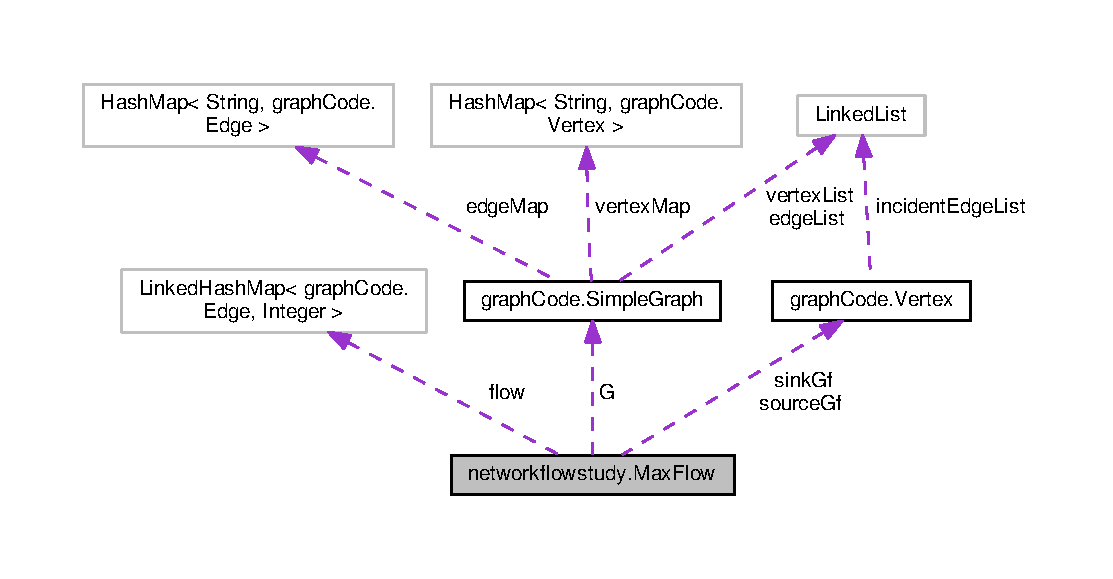
\includegraphics[width=350pt]{classnetworkflowstudy_1_1MaxFlow__coll__graph}
\end{center}
\end{figure}
\subsection*{Public Member Functions}
\begin{DoxyCompactItemize}
\item 
{\bfseries Max\+Flow} (\hyperlink{classgraphCode_1_1SimpleGraph}{Simple\+Graph} G)\hypertarget{classnetworkflowstudy_1_1MaxFlow_a117178d28cedbcc7ff80b2bb6e160b29}{}\label{classnetworkflowstudy_1_1MaxFlow_a117178d28cedbcc7ff80b2bb6e160b29}

\item 
Linked\+Hash\+Map$<$ \hyperlink{classgraphCode_1_1Edge}{Edge}, Integer $>$ \hyperlink{classnetworkflowstudy_1_1MaxFlow_af4305363e5a4a606d03af69726bc00f9}{calculate\+Flow} (\hyperlink{classgraphCode_1_1Vertex}{Vertex} sourceG, \hyperlink{classgraphCode_1_1Vertex}{Vertex} sinkG)
\end{DoxyCompactItemize}


\subsection{Detailed Description}
Calculates the max Flow using Ford Fulkerson \begin{DoxyAuthor}{Author}
bhagatsanchya 
\end{DoxyAuthor}


\subsection{Member Function Documentation}
\index{networkflowstudy\+::\+Max\+Flow@{networkflowstudy\+::\+Max\+Flow}!calculate\+Flow@{calculate\+Flow}}
\index{calculate\+Flow@{calculate\+Flow}!networkflowstudy\+::\+Max\+Flow@{networkflowstudy\+::\+Max\+Flow}}
\subsubsection[{\texorpdfstring{calculate\+Flow(\+Vertex source\+G, Vertex sink\+G)}{calculateFlow(Vertex sourceG, Vertex sinkG)}}]{\setlength{\rightskip}{0pt plus 5cm}Linked\+Hash\+Map$<${\bf Edge}, Integer$>$ networkflowstudy.\+Max\+Flow.\+calculate\+Flow (
\begin{DoxyParamCaption}
\item[{{\bf Vertex}}]{sourceG, }
\item[{{\bf Vertex}}]{sinkG}
\end{DoxyParamCaption}
)\hspace{0.3cm}{\ttfamily [inline]}}\hypertarget{classnetworkflowstudy_1_1MaxFlow_af4305363e5a4a606d03af69726bc00f9}{}\label{classnetworkflowstudy_1_1MaxFlow_af4305363e5a4a606d03af69726bc00f9}
Calculate flow of a network using Ford fulkerson max-\/ flow algorithm 
\begin{DoxyParams}{Parameters}
{\em sourceG} & vertex sourceG \\
\hline
{\em sinkG} & vertex sinkG \\
\hline
\end{DoxyParams}
\begin{DoxyReturn}{Returns}
flow 
\end{DoxyReturn}


The documentation for this class was generated from the following file\+:\begin{DoxyCompactItemize}
\item 
/home/anisha/\+Algo\+Project/\+Network\+Flow\+Study/src/networkflowstudy/Max\+Flow.\+java\end{DoxyCompactItemize}

\hypertarget{classgraphGenerationCode_1_1Mesh_1_1MeshGenerator}{}\section{graph\+Generation\+Code.\+Mesh.\+Mesh\+Generator Class Reference}
\label{classgraphGenerationCode_1_1Mesh_1_1MeshGenerator}\index{graph\+Generation\+Code.\+Mesh.\+Mesh\+Generator@{graph\+Generation\+Code.\+Mesh.\+Mesh\+Generator}}
\subsection*{Public Member Functions}
\begin{DoxyCompactItemize}
\item 
void \hyperlink{classgraphGenerationCode_1_1Mesh_1_1MeshGenerator_a4658a0e6ef335d61aaad0951e7bea550}{generate} ()
\item 
\hyperlink{classgraphGenerationCode_1_1Mesh_1_1MeshGenerator_a50aaa5dc64717b0685b7d744bd336580}{Mesh\+Generator} (String\mbox{[}$\,$\mbox{]} args)
\end{DoxyCompactItemize}
\subsection*{Static Public Member Functions}
\begin{DoxyCompactItemize}
\item 
static void \hyperlink{classgraphGenerationCode_1_1Mesh_1_1MeshGenerator_ad5644a452d15eb4cd640dfb1c1c0d2c9}{main} (String\mbox{[}$\,$\mbox{]} args)
\end{DoxyCompactItemize}


\subsection{Detailed Description}
This class generates text files representing mesh graph flow networks. The mesh graphs have edges from s to each node in the first column, from each internal node to the node on its right, both ways between every internal node and the nodes above and below it, and from the last column nodes to the sink.

The file format is the standard T\+C\+SS 343/543 format of \textquotesingle{}first vertex\textquotesingle{} \textquotesingle{}second vertex\textquotesingle{} \textquotesingle{}capacity\textquotesingle{}. The program takes command line arguments. They are\+: \mbox{[}\# of rows\mbox{]} \mbox{[}\# of columns\mbox{]}\mbox{[}capacity or maximum capacity\mbox{]}\mbox{[}filename\mbox{]}\mbox{[}-\/cc flag\mbox{]}. All arguments are optional. If you enter no arguments, you get a 3 x 4 mesh with capacity of 1 on all edges, printed to System.\+out. The arguments are\+:

\#rows/columns -\/ self-\/explanatory...defaults to 3x4 if no arguments are given

capacity -\/ defaults to 1(fixed) if $<$3 arguments. Otherwise random on the range 1 to capacity, unless \textquotesingle{}-\/cc\textquotesingle{} set.

filename -\/ the name of file to write to. Defaults to System.\+out if $<$4 parameters (or if -\/cc is last parameter)

-\/cc flag...With at least the first three parameters specified, ending the line with \textquotesingle{}-\/cc\textquotesingle{} will cause edge capacities to have a constant value of c.

\begin{DoxyAuthor}{Author}
T\+C\+SS 543 group 2\+: Apaporn Boonyaratta, Richard Hill, Quang Lu, \& David Thaler 
\end{DoxyAuthor}
\begin{DoxyVersion}{Version}
November 21, 2008 
\end{DoxyVersion}


\subsection{Constructor \& Destructor Documentation}
\index{graph\+Generation\+Code\+::\+Mesh\+::\+Mesh\+Generator@{graph\+Generation\+Code\+::\+Mesh\+::\+Mesh\+Generator}!Mesh\+Generator@{Mesh\+Generator}}
\index{Mesh\+Generator@{Mesh\+Generator}!graph\+Generation\+Code\+::\+Mesh\+::\+Mesh\+Generator@{graph\+Generation\+Code\+::\+Mesh\+::\+Mesh\+Generator}}
\subsubsection[{\texorpdfstring{Mesh\+Generator(\+String[] args)}{MeshGenerator(String[] args)}}]{\setlength{\rightskip}{0pt plus 5cm}graph\+Generation\+Code.\+Mesh.\+Mesh\+Generator.\+Mesh\+Generator (
\begin{DoxyParamCaption}
\item[{String\mbox{[}$\,$\mbox{]}}]{args}
\end{DoxyParamCaption}
)\hspace{0.3cm}{\ttfamily [inline]}}\hypertarget{classgraphGenerationCode_1_1Mesh_1_1MeshGenerator_a50aaa5dc64717b0685b7d744bd336580}{}\label{classgraphGenerationCode_1_1Mesh_1_1MeshGenerator_a50aaa5dc64717b0685b7d744bd336580}
Constructor for mesh generator parses the command line arguments and sets the defaults. See the class comment for arguments/defaults.


\begin{DoxyParams}{Parameters}
{\em args} & -\/ the command line arguments. See class comment. \\
\hline
\end{DoxyParams}


\subsection{Member Function Documentation}
\index{graph\+Generation\+Code\+::\+Mesh\+::\+Mesh\+Generator@{graph\+Generation\+Code\+::\+Mesh\+::\+Mesh\+Generator}!generate@{generate}}
\index{generate@{generate}!graph\+Generation\+Code\+::\+Mesh\+::\+Mesh\+Generator@{graph\+Generation\+Code\+::\+Mesh\+::\+Mesh\+Generator}}
\subsubsection[{\texorpdfstring{generate()}{generate()}}]{\setlength{\rightskip}{0pt plus 5cm}void graph\+Generation\+Code.\+Mesh.\+Mesh\+Generator.\+generate (
\begin{DoxyParamCaption}
{}
\end{DoxyParamCaption}
)\hspace{0.3cm}{\ttfamily [inline]}}\hypertarget{classgraphGenerationCode_1_1Mesh_1_1MeshGenerator_a4658a0e6ef335d61aaad0951e7bea550}{}\label{classgraphGenerationCode_1_1Mesh_1_1MeshGenerator_a4658a0e6ef335d61aaad0951e7bea550}
The run method. \index{graph\+Generation\+Code\+::\+Mesh\+::\+Mesh\+Generator@{graph\+Generation\+Code\+::\+Mesh\+::\+Mesh\+Generator}!main@{main}}
\index{main@{main}!graph\+Generation\+Code\+::\+Mesh\+::\+Mesh\+Generator@{graph\+Generation\+Code\+::\+Mesh\+::\+Mesh\+Generator}}
\subsubsection[{\texorpdfstring{main(\+String[] args)}{main(String[] args)}}]{\setlength{\rightskip}{0pt plus 5cm}static void graph\+Generation\+Code.\+Mesh.\+Mesh\+Generator.\+main (
\begin{DoxyParamCaption}
\item[{String\mbox{[}$\,$\mbox{]}}]{args}
\end{DoxyParamCaption}
)\hspace{0.3cm}{\ttfamily [inline]}, {\ttfamily [static]}}\hypertarget{classgraphGenerationCode_1_1Mesh_1_1MeshGenerator_ad5644a452d15eb4cd640dfb1c1c0d2c9}{}\label{classgraphGenerationCode_1_1Mesh_1_1MeshGenerator_ad5644a452d15eb4cd640dfb1c1c0d2c9}

\begin{DoxyParams}{Parameters}
{\em args-\/} & command line args \\
\hline
\end{DoxyParams}


The documentation for this class was generated from the following file\+:\begin{DoxyCompactItemize}
\item 
/home/anisha/\+Algo\+Project/\+Network\+Flow\+Study/src/graph\+Generation\+Code/\+Mesh/Mesh\+Generator.\+java\end{DoxyCompactItemize}

\hypertarget{classnetworkflowstudy_1_1PreflowPush}{}\section{networkflowstudy.\+Preflow\+Push Class Reference}
\label{classnetworkflowstudy_1_1PreflowPush}\index{networkflowstudy.\+Preflow\+Push@{networkflowstudy.\+Preflow\+Push}}


Collaboration diagram for networkflowstudy.\+Preflow\+Push\+:\nopagebreak
\begin{figure}[H]
\begin{center}
\leavevmode
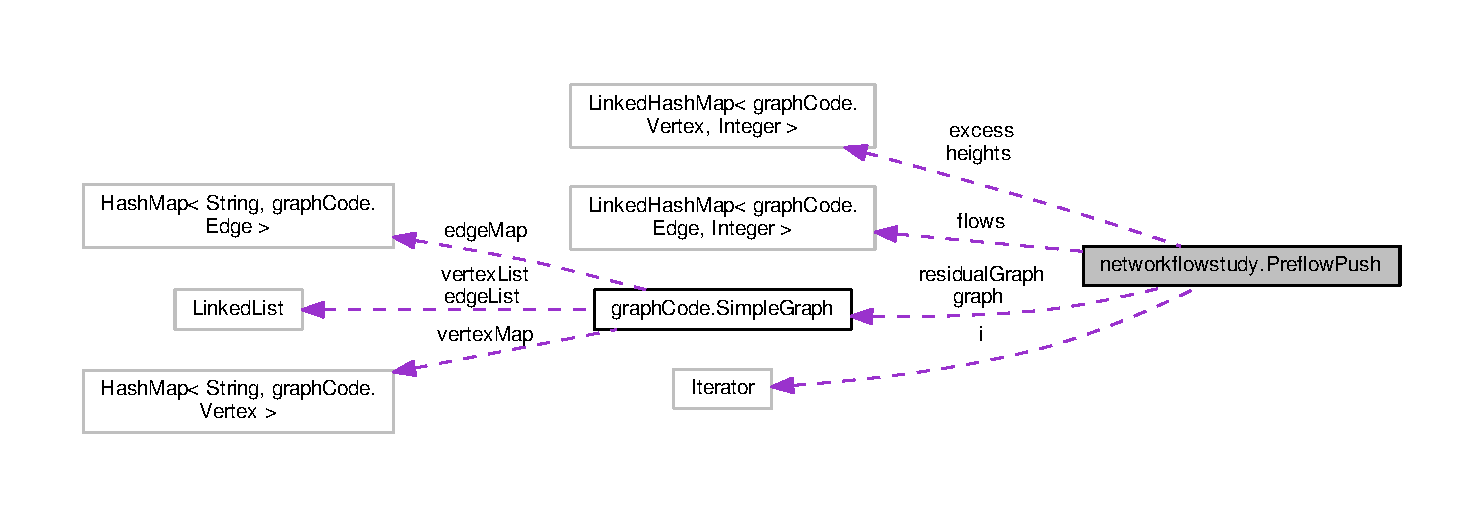
\includegraphics[width=350pt]{classnetworkflowstudy_1_1PreflowPush__coll__graph}
\end{center}
\end{figure}
\subsection*{Public Member Functions}
\begin{Indent}{\bf Constructor}\par
{\em 
\begin{DoxyParams}{Parameters}
{\em g} & represents a Simple\+Graph to find max flow for. \\
\hline
\end{DoxyParams}
}\begin{DoxyCompactItemize}
\item 
{\bfseries Preflow\+Push} (\hyperlink{classgraphCode_1_1SimpleGraph}{Simple\+Graph} g)\hypertarget{classnetworkflowstudy_1_1PreflowPush_a509ad952e5697ec0ad3109bc09b97e50}{}\label{classnetworkflowstudy_1_1PreflowPush_a509ad952e5697ec0ad3109bc09b97e50}

\end{DoxyCompactItemize}
\end{Indent}
\begin{Indent}{\bf Get\+Max\+Flow}\par
{\em \begin{DoxyReturn}{Returns}
the flow of the graph in a linked hash map of Edge to Integer. 
\end{DoxyReturn}
}\begin{DoxyCompactItemize}
\item 
Linked\+Hash\+Map$<$ \hyperlink{classgraphCode_1_1Edge}{Edge}, Integer $>$ {\bfseries Get\+Max\+Flow} ()\hypertarget{classnetworkflowstudy_1_1PreflowPush_abd0c41b475ef9df44b22a0fe4c31474a}{}\label{classnetworkflowstudy_1_1PreflowPush_abd0c41b475ef9df44b22a0fe4c31474a}

\end{DoxyCompactItemize}
\end{Indent}


\subsection{Detailed Description}
\begin{DoxyAuthor}{Author}
jason 
\end{DoxyAuthor}


The documentation for this class was generated from the following file\+:\begin{DoxyCompactItemize}
\item 
/home/anisha/\+Algo\+Project/\+Network\+Flow\+Study/src/networkflowstudy/Preflow\+Push.\+java\end{DoxyCompactItemize}

\hypertarget{classRandomGraph}{}\section{Random\+Graph Class Reference}
\label{classRandomGraph}\index{Random\+Graph@{Random\+Graph}}
\subsection*{Static Public Member Functions}
\begin{DoxyCompactItemize}
\item 
static void \hyperlink{classRandomGraph_a2593e0cde132ce52aa89d66209b05185}{main} (String\mbox{[}$\,$\mbox{]} args)
\item 
static String\+Buffer \hyperlink{classRandomGraph_afaceccd1b746cf18dabf4d7a430cf710}{graph\+Builder} (int v, int e, int min, int max)
\end{DoxyCompactItemize}


\subsection{Member Function Documentation}
\index{Random\+Graph@{Random\+Graph}!graph\+Builder@{graph\+Builder}}
\index{graph\+Builder@{graph\+Builder}!Random\+Graph@{Random\+Graph}}
\subsubsection[{\texorpdfstring{graph\+Builder(int v, int e, int min, int max)}{graphBuilder(int v, int e, int min, int max)}}]{\setlength{\rightskip}{0pt plus 5cm}static String\+Buffer Random\+Graph.\+graph\+Builder (
\begin{DoxyParamCaption}
\item[{int}]{v, }
\item[{int}]{e, }
\item[{int}]{min, }
\item[{int}]{max}
\end{DoxyParamCaption}
)\hspace{0.3cm}{\ttfamily [inline]}, {\ttfamily [static]}}\hypertarget{classRandomGraph_afaceccd1b746cf18dabf4d7a430cf710}{}\label{classRandomGraph_afaceccd1b746cf18dabf4d7a430cf710}
This method creates a 3 token representation of a graph. 
\begin{DoxyParams}{Parameters}
{\em v} & The number of vertices in the graph \\
\hline
{\em e} & The number of edges leaving each vertice \\
\hline
{\em min} & The lowerbound on the capacity value of each edge \\
\hline
{\em max} & The upperbound on the capacity value of each edge \\
\hline
\end{DoxyParams}
\begin{DoxyReturn}{Returns}
A string buffer, each line contains 3 tokens corresponding to a directed edge\+: the tail, the head, and the capacity. 
\end{DoxyReturn}
\index{Random\+Graph@{Random\+Graph}!main@{main}}
\index{main@{main}!Random\+Graph@{Random\+Graph}}
\subsubsection[{\texorpdfstring{main(\+String[] args)}{main(String[] args)}}]{\setlength{\rightskip}{0pt plus 5cm}static void Random\+Graph.\+main (
\begin{DoxyParamCaption}
\item[{String\mbox{[}$\,$\mbox{]}}]{args}
\end{DoxyParamCaption}
)\hspace{0.3cm}{\ttfamily [inline]}, {\ttfamily [static]}}\hypertarget{classRandomGraph_a2593e0cde132ce52aa89d66209b05185}{}\label{classRandomGraph_a2593e0cde132ce52aa89d66209b05185}
Entrance point for the program. java \hyperlink{classRandomGraph}{Random\+Graph} v, e, m, f 
\begin{DoxyParams}{Parameters}
{\em v} & -\/ the number of vertices \\
\hline
{\em e} & -\/ the number of edges leaving each node \\
\hline
{\em min} & -\/ the lower bound on the edge capacities \\
\hline
{\em max} & -\/ the upper bound on the edge capacities \\
\hline
{\em f} & -\/ path and file name for saving the graph \\
\hline
\end{DoxyParams}


The documentation for this class was generated from the following file\+:\begin{DoxyCompactItemize}
\item 
/home/anisha/\+Algo\+Project/\+Network\+Flow\+Study/src/graph\+Generation\+Code/\+Fixed\+Degree/Random\+Graph.\+java\end{DoxyCompactItemize}

\hypertarget{classnetworkflowstudy_1_1SaveOutput}{}\section{networkflowstudy.\+Save\+Output Class Reference}
\label{classnetworkflowstudy_1_1SaveOutput}\index{networkflowstudy.\+Save\+Output@{networkflowstudy.\+Save\+Output}}
\subsection*{Static Public Member Functions}
\begin{DoxyCompactItemize}
\item 
static void {\bfseries write\+To\+C\+SV} (String graph\+Type, String algorithm\+Name, int number\+Of\+Vertices, long running\+Time, int max\+Flow)  throws I\+O\+Exception \hypertarget{classnetworkflowstudy_1_1SaveOutput_a9c8e9fa3b7f273f6b63025dd4afea9e5}{}\label{classnetworkflowstudy_1_1SaveOutput_a9c8e9fa3b7f273f6b63025dd4afea9e5}

\item 
static void {\bfseries write\+To\+C\+SV} (String graph\+Type, String algorithm\+Name, int number\+Of\+Vertices, long running\+Time, int max\+Flow, int capacity)  throws I\+O\+Exception \hypertarget{classnetworkflowstudy_1_1SaveOutput_a9004b849510ac57e5e9f4fd6dfd9308f}{}\label{classnetworkflowstudy_1_1SaveOutput_a9004b849510ac57e5e9f4fd6dfd9308f}

\end{DoxyCompactItemize}


\subsection{Detailed Description}
\begin{DoxyAuthor}{Author}
anisha 
\end{DoxyAuthor}


The documentation for this class was generated from the following file\+:\begin{DoxyCompactItemize}
\item 
/home/anisha/\+Algo\+Project/\+Network\+Flow\+Study/src/networkflowstudy/Save\+Output.\+java\end{DoxyCompactItemize}

\hypertarget{classnetworkflowstudy_1_1ScalingMaxFlow}{}\section{networkflowstudy.\+Scaling\+Max\+Flow Class Reference}
\label{classnetworkflowstudy_1_1ScalingMaxFlow}\index{networkflowstudy.\+Scaling\+Max\+Flow@{networkflowstudy.\+Scaling\+Max\+Flow}}


Collaboration diagram for networkflowstudy.\+Scaling\+Max\+Flow\+:\nopagebreak
\begin{figure}[H]
\begin{center}
\leavevmode
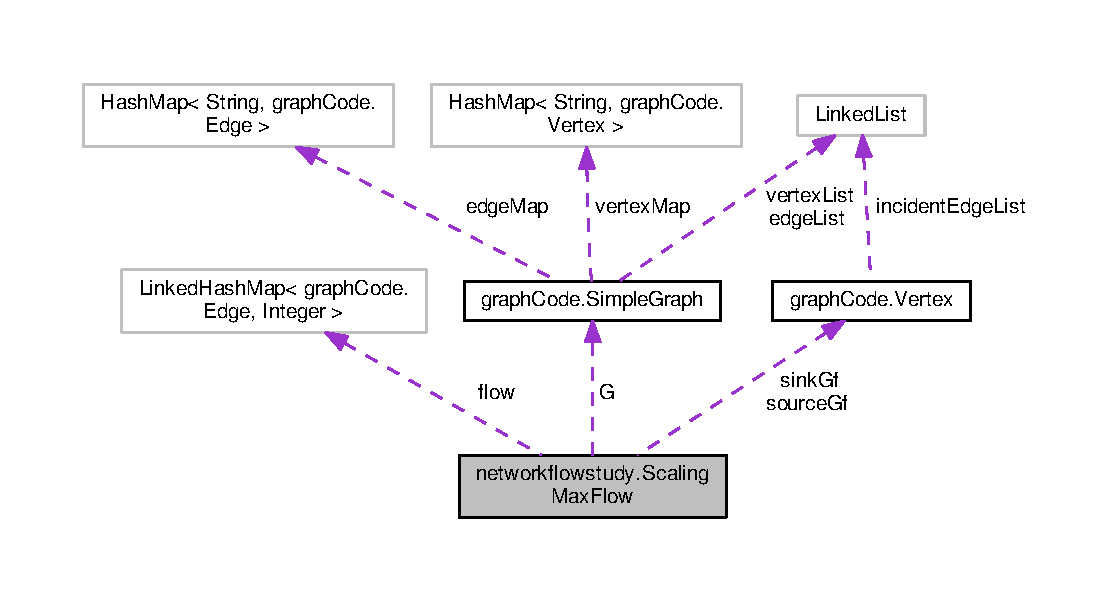
\includegraphics[width=350pt]{classnetworkflowstudy_1_1ScalingMaxFlow__coll__graph}
\end{center}
\end{figure}
\subsection*{Public Member Functions}
\begin{DoxyCompactItemize}
\item 
\hyperlink{classnetworkflowstudy_1_1ScalingMaxFlow_a5f44980b9bf6c85fc0b925c5527e3464}{Scaling\+Max\+Flow} (\hyperlink{classgraphCode_1_1SimpleGraph}{Simple\+Graph} G)
\item 
Linked\+Hash\+Map$<$ \hyperlink{classgraphCode_1_1Edge}{Edge}, Integer $>$ \hyperlink{classnetworkflowstudy_1_1ScalingMaxFlow_a14309c02ceb7dc345452eced38777696}{calculate\+Flow} (\hyperlink{classgraphCode_1_1Vertex}{Vertex} sourceG, \hyperlink{classgraphCode_1_1Vertex}{Vertex} sinkG)
\item 
int \hyperlink{classnetworkflowstudy_1_1ScalingMaxFlow_a5d2651a2301430ad246aea848eb34a91}{get\+Delta} (\hyperlink{classgraphCode_1_1Vertex}{Vertex} source)
\end{DoxyCompactItemize}


\subsection{Detailed Description}
Calculates and returns flow using Scaling max Flow algorithm \begin{DoxyAuthor}{Author}
anisha 
\end{DoxyAuthor}


\subsection{Constructor \& Destructor Documentation}
\index{networkflowstudy\+::\+Scaling\+Max\+Flow@{networkflowstudy\+::\+Scaling\+Max\+Flow}!Scaling\+Max\+Flow@{Scaling\+Max\+Flow}}
\index{Scaling\+Max\+Flow@{Scaling\+Max\+Flow}!networkflowstudy\+::\+Scaling\+Max\+Flow@{networkflowstudy\+::\+Scaling\+Max\+Flow}}
\subsubsection[{\texorpdfstring{Scaling\+Max\+Flow(\+Simple\+Graph G)}{ScalingMaxFlow(SimpleGraph G)}}]{\setlength{\rightskip}{0pt plus 5cm}networkflowstudy.\+Scaling\+Max\+Flow.\+Scaling\+Max\+Flow (
\begin{DoxyParamCaption}
\item[{{\bf Simple\+Graph}}]{G}
\end{DoxyParamCaption}
)\hspace{0.3cm}{\ttfamily [inline]}}\hypertarget{classnetworkflowstudy_1_1ScalingMaxFlow_a5f44980b9bf6c85fc0b925c5527e3464}{}\label{classnetworkflowstudy_1_1ScalingMaxFlow_a5f44980b9bf6c85fc0b925c5527e3464}
Constructor to initialize the flow along all edges and create the corresponding graph 
\begin{DoxyParams}{Parameters}
{\em G} & \\
\hline
\end{DoxyParams}


\subsection{Member Function Documentation}
\index{networkflowstudy\+::\+Scaling\+Max\+Flow@{networkflowstudy\+::\+Scaling\+Max\+Flow}!calculate\+Flow@{calculate\+Flow}}
\index{calculate\+Flow@{calculate\+Flow}!networkflowstudy\+::\+Scaling\+Max\+Flow@{networkflowstudy\+::\+Scaling\+Max\+Flow}}
\subsubsection[{\texorpdfstring{calculate\+Flow(\+Vertex source\+G, Vertex sink\+G)}{calculateFlow(Vertex sourceG, Vertex sinkG)}}]{\setlength{\rightskip}{0pt plus 5cm}Linked\+Hash\+Map$<${\bf Edge}, Integer$>$ networkflowstudy.\+Scaling\+Max\+Flow.\+calculate\+Flow (
\begin{DoxyParamCaption}
\item[{{\bf Vertex}}]{sourceG, }
\item[{{\bf Vertex}}]{sinkG}
\end{DoxyParamCaption}
)\hspace{0.3cm}{\ttfamily [inline]}}\hypertarget{classnetworkflowstudy_1_1ScalingMaxFlow_a14309c02ceb7dc345452eced38777696}{}\label{classnetworkflowstudy_1_1ScalingMaxFlow_a14309c02ceb7dc345452eced38777696}
Calculate flow of a network using Scaling max-\/ flow algorithm 
\begin{DoxyParams}{Parameters}
{\em source} & vertex sourceG \\
\hline
{\em sink} & vertex sinkG \\
\hline
\end{DoxyParams}
\begin{DoxyReturn}{Returns}
flow 
\end{DoxyReturn}
\index{networkflowstudy\+::\+Scaling\+Max\+Flow@{networkflowstudy\+::\+Scaling\+Max\+Flow}!get\+Delta@{get\+Delta}}
\index{get\+Delta@{get\+Delta}!networkflowstudy\+::\+Scaling\+Max\+Flow@{networkflowstudy\+::\+Scaling\+Max\+Flow}}
\subsubsection[{\texorpdfstring{get\+Delta(\+Vertex source)}{getDelta(Vertex source)}}]{\setlength{\rightskip}{0pt plus 5cm}int networkflowstudy.\+Scaling\+Max\+Flow.\+get\+Delta (
\begin{DoxyParamCaption}
\item[{{\bf Vertex}}]{source}
\end{DoxyParamCaption}
)\hspace{0.3cm}{\ttfamily [inline]}}\hypertarget{classnetworkflowstudy_1_1ScalingMaxFlow_a5d2651a2301430ad246aea848eb34a91}{}\label{classnetworkflowstudy_1_1ScalingMaxFlow_a5d2651a2301430ad246aea848eb34a91}
calculate delta for a residual graph G 
\begin{DoxyParams}{Parameters}
{\em source} & vertex in residual graph \\
\hline
\end{DoxyParams}
\begin{DoxyReturn}{Returns}
delta 
\end{DoxyReturn}


The documentation for this class was generated from the following file\+:\begin{DoxyCompactItemize}
\item 
/home/anisha/\+Algo\+Project/\+Network\+Flow\+Study/src/networkflowstudy/Scaling\+Max\+Flow.\+java\end{DoxyCompactItemize}

\hypertarget{classgraphCode_1_1SimpleGraph}{}\section{graph\+Code.\+Simple\+Graph Class Reference}
\label{classgraphCode_1_1SimpleGraph}\index{graph\+Code.\+Simple\+Graph@{graph\+Code.\+Simple\+Graph}}


Collaboration diagram for graph\+Code.\+Simple\+Graph\+:\nopagebreak
\begin{figure}[H]
\begin{center}
\leavevmode
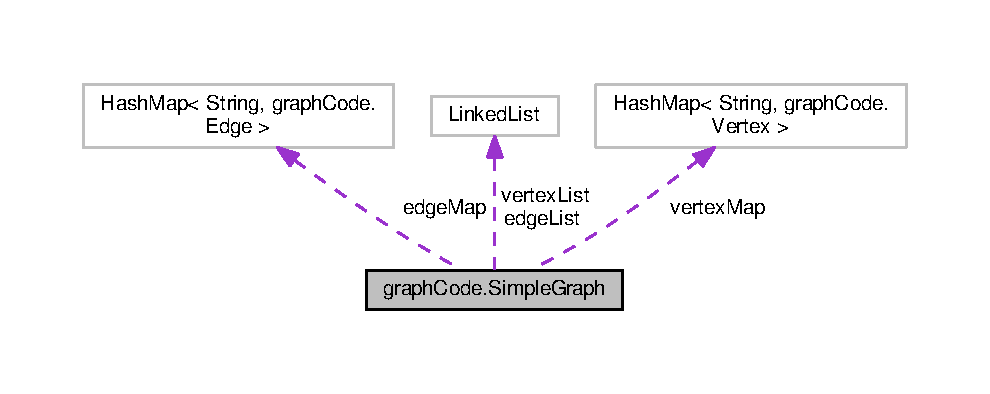
\includegraphics[width=350pt]{classgraphCode_1_1SimpleGraph__coll__graph}
\end{center}
\end{figure}
\subsection*{Public Member Functions}
\begin{DoxyCompactItemize}
\item 
Iterator \hyperlink{classgraphCode_1_1SimpleGraph_a9c8e1eedfc1f1f9b15cbaf0b7d1e60cd}{vertices} ()
\item 
Iterator \hyperlink{classgraphCode_1_1SimpleGraph_a806589f8bd826802e960c2cc3e6d7c06}{edges} ()
\item 
Hash\+Map \hyperlink{classgraphCode_1_1SimpleGraph_a3abf29703b8e059453d3c11da066dd25}{get\+Vertex\+Map} ()
\item 
Hash\+Map \hyperlink{classgraphCode_1_1SimpleGraph_a2f70f56636e2d881b2593760453d4723}{get\+Edge\+Map} ()
\item 
Iterator \hyperlink{classgraphCode_1_1SimpleGraph_a1c8b377618c14bed26e8007e9b23eda5}{incident\+Edges} (\hyperlink{classgraphCode_1_1Vertex}{Vertex} v)
\item 
\hyperlink{classgraphCode_1_1Vertex}{Vertex} \hyperlink{classgraphCode_1_1SimpleGraph_a4348702804a838f36d7515a765ea8389}{a\+Vertex} ()
\item 
\hyperlink{classgraphCode_1_1Vertex}{Vertex} \hyperlink{classgraphCode_1_1SimpleGraph_a5c1202dd0060fd97620c1dfe4184a371}{insert\+Vertex} (Object data, Object name)
\item 
\hyperlink{classgraphCode_1_1Edge}{Edge} \hyperlink{classgraphCode_1_1SimpleGraph_a4507c310762a6091a25e8cd922662d7e}{insert\+Edge} (\hyperlink{classgraphCode_1_1Vertex}{Vertex} v, \hyperlink{classgraphCode_1_1Vertex}{Vertex} w, Object data, Object name)
\item 
\hyperlink{classgraphCode_1_1Vertex}{Vertex} \hyperlink{classgraphCode_1_1SimpleGraph_ad700bce03aa2ab5cb067a9c5feb2f049}{opposite} (\hyperlink{classgraphCode_1_1Vertex}{Vertex} v, \hyperlink{classgraphCode_1_1Edge}{Edge} e)
\item 
\hyperlink{classgraphCode_1_1Vertex}{Vertex} \hyperlink{classgraphCode_1_1SimpleGraph_a2537a9016af6f2509381c124ed3de524}{tail} (\hyperlink{classgraphCode_1_1Vertex}{Vertex} v, \hyperlink{classgraphCode_1_1Edge}{Edge} e)
\item 
int \hyperlink{classgraphCode_1_1SimpleGraph_ac00393b0333d8b19f2581c4773b8451e}{num\+Vertices} ()
\item 
int \hyperlink{classgraphCode_1_1SimpleGraph_a11a7c6c52ebf307077ab6b887c122425}{num\+Edges} ()
\item 
\hyperlink{classgraphCode_1_1Vertex}{Vertex} \hyperlink{classgraphCode_1_1SimpleGraph_aab1ec8273dce11b72f198ce45ce1e866}{get\+Vertex} (String vertex\+Name)
\end{DoxyCompactItemize}
\subsection*{Static Public Member Functions}
\begin{DoxyCompactItemize}
\item 
static void \hyperlink{classgraphCode_1_1SimpleGraph_a6368cc5b7180cd0d7aafb0f315b944f6}{main} (String\mbox{[}$\,$\mbox{]} args)
\end{DoxyCompactItemize}


\subsection{Detailed Description}
A class that represents a graph.

\begin{DoxyAuthor}{Author}
edhong 
\end{DoxyAuthor}
\begin{DoxyVersion}{Version}
0.\+0 
\end{DoxyVersion}


\subsection{Member Function Documentation}
\index{graph\+Code\+::\+Simple\+Graph@{graph\+Code\+::\+Simple\+Graph}!a\+Vertex@{a\+Vertex}}
\index{a\+Vertex@{a\+Vertex}!graph\+Code\+::\+Simple\+Graph@{graph\+Code\+::\+Simple\+Graph}}
\subsubsection[{\texorpdfstring{a\+Vertex()}{aVertex()}}]{\setlength{\rightskip}{0pt plus 5cm}{\bf Vertex} graph\+Code.\+Simple\+Graph.\+a\+Vertex (
\begin{DoxyParamCaption}
{}
\end{DoxyParamCaption}
)\hspace{0.3cm}{\ttfamily [inline]}}\hypertarget{classgraphCode_1_1SimpleGraph_a4348702804a838f36d7515a765ea8389}{}\label{classgraphCode_1_1SimpleGraph_a4348702804a838f36d7515a765ea8389}
Return an arbitrary vertex of this graph \begin{DoxyReturn}{Returns}
some vertex of this graph 
\end{DoxyReturn}
\index{graph\+Code\+::\+Simple\+Graph@{graph\+Code\+::\+Simple\+Graph}!edges@{edges}}
\index{edges@{edges}!graph\+Code\+::\+Simple\+Graph@{graph\+Code\+::\+Simple\+Graph}}
\subsubsection[{\texorpdfstring{edges()}{edges()}}]{\setlength{\rightskip}{0pt plus 5cm}Iterator graph\+Code.\+Simple\+Graph.\+edges (
\begin{DoxyParamCaption}
{}
\end{DoxyParamCaption}
)\hspace{0.3cm}{\ttfamily [inline]}}\hypertarget{classgraphCode_1_1SimpleGraph_a806589f8bd826802e960c2cc3e6d7c06}{}\label{classgraphCode_1_1SimpleGraph_a806589f8bd826802e960c2cc3e6d7c06}
Return the edge list of this graph. \begin{DoxyReturn}{Returns}
edge list of this graph 
\end{DoxyReturn}
\index{graph\+Code\+::\+Simple\+Graph@{graph\+Code\+::\+Simple\+Graph}!get\+Edge\+Map@{get\+Edge\+Map}}
\index{get\+Edge\+Map@{get\+Edge\+Map}!graph\+Code\+::\+Simple\+Graph@{graph\+Code\+::\+Simple\+Graph}}
\subsubsection[{\texorpdfstring{get\+Edge\+Map()}{getEdgeMap()}}]{\setlength{\rightskip}{0pt plus 5cm}Hash\+Map graph\+Code.\+Simple\+Graph.\+get\+Edge\+Map (
\begin{DoxyParamCaption}
{}
\end{DoxyParamCaption}
)\hspace{0.3cm}{\ttfamily [inline]}}\hypertarget{classgraphCode_1_1SimpleGraph_a2f70f56636e2d881b2593760453d4723}{}\label{classgraphCode_1_1SimpleGraph_a2f70f56636e2d881b2593760453d4723}
get graph edge hash\+Map \begin{DoxyReturn}{Returns}
edge\+Map 
\end{DoxyReturn}
\index{graph\+Code\+::\+Simple\+Graph@{graph\+Code\+::\+Simple\+Graph}!get\+Vertex@{get\+Vertex}}
\index{get\+Vertex@{get\+Vertex}!graph\+Code\+::\+Simple\+Graph@{graph\+Code\+::\+Simple\+Graph}}
\subsubsection[{\texorpdfstring{get\+Vertex(\+String vertex\+Name)}{getVertex(String vertexName)}}]{\setlength{\rightskip}{0pt plus 5cm}{\bf Vertex} graph\+Code.\+Simple\+Graph.\+get\+Vertex (
\begin{DoxyParamCaption}
\item[{String}]{vertex\+Name}
\end{DoxyParamCaption}
)\hspace{0.3cm}{\ttfamily [inline]}}\hypertarget{classgraphCode_1_1SimpleGraph_aab1ec8273dce11b72f198ce45ce1e866}{}\label{classgraphCode_1_1SimpleGraph_aab1ec8273dce11b72f198ce45ce1e866}
Returns the vertex in a given \hyperlink{classgraphCode_1_1SimpleGraph}{Simple\+Graph} object 
\begin{DoxyParams}{Parameters}
{\em vertex\+Name} & \\
\hline
\end{DoxyParams}
\begin{DoxyReturn}{Returns}
source vertex 
\end{DoxyReturn}
\index{graph\+Code\+::\+Simple\+Graph@{graph\+Code\+::\+Simple\+Graph}!get\+Vertex\+Map@{get\+Vertex\+Map}}
\index{get\+Vertex\+Map@{get\+Vertex\+Map}!graph\+Code\+::\+Simple\+Graph@{graph\+Code\+::\+Simple\+Graph}}
\subsubsection[{\texorpdfstring{get\+Vertex\+Map()}{getVertexMap()}}]{\setlength{\rightskip}{0pt plus 5cm}Hash\+Map graph\+Code.\+Simple\+Graph.\+get\+Vertex\+Map (
\begin{DoxyParamCaption}
{}
\end{DoxyParamCaption}
)\hspace{0.3cm}{\ttfamily [inline]}}\hypertarget{classgraphCode_1_1SimpleGraph_a3abf29703b8e059453d3c11da066dd25}{}\label{classgraphCode_1_1SimpleGraph_a3abf29703b8e059453d3c11da066dd25}
get graph vertex hash\+Map \begin{DoxyReturn}{Returns}
vertex\+Map 
\end{DoxyReturn}
\index{graph\+Code\+::\+Simple\+Graph@{graph\+Code\+::\+Simple\+Graph}!incident\+Edges@{incident\+Edges}}
\index{incident\+Edges@{incident\+Edges}!graph\+Code\+::\+Simple\+Graph@{graph\+Code\+::\+Simple\+Graph}}
\subsubsection[{\texorpdfstring{incident\+Edges(\+Vertex v)}{incidentEdges(Vertex v)}}]{\setlength{\rightskip}{0pt plus 5cm}Iterator graph\+Code.\+Simple\+Graph.\+incident\+Edges (
\begin{DoxyParamCaption}
\item[{{\bf Vertex}}]{v}
\end{DoxyParamCaption}
)\hspace{0.3cm}{\ttfamily [inline]}}\hypertarget{classgraphCode_1_1SimpleGraph_a1c8b377618c14bed26e8007e9b23eda5}{}\label{classgraphCode_1_1SimpleGraph_a1c8b377618c14bed26e8007e9b23eda5}
Given a vertex, return an iterator to the edge list of that vertex 
\begin{DoxyParams}{Parameters}
{\em v} & a vertex \\
\hline
\end{DoxyParams}
\begin{DoxyReturn}{Returns}
an iterator to the edge list of that vertex 
\end{DoxyReturn}
\index{graph\+Code\+::\+Simple\+Graph@{graph\+Code\+::\+Simple\+Graph}!insert\+Edge@{insert\+Edge}}
\index{insert\+Edge@{insert\+Edge}!graph\+Code\+::\+Simple\+Graph@{graph\+Code\+::\+Simple\+Graph}}
\subsubsection[{\texorpdfstring{insert\+Edge(\+Vertex v, Vertex w, Object data, Object name)}{insertEdge(Vertex v, Vertex w, Object data, Object name)}}]{\setlength{\rightskip}{0pt plus 5cm}{\bf Edge} graph\+Code.\+Simple\+Graph.\+insert\+Edge (
\begin{DoxyParamCaption}
\item[{{\bf Vertex}}]{v, }
\item[{{\bf Vertex}}]{w, }
\item[{Object}]{data, }
\item[{Object}]{name}
\end{DoxyParamCaption}
)\hspace{0.3cm}{\ttfamily [inline]}}\hypertarget{classgraphCode_1_1SimpleGraph_a4507c310762a6091a25e8cd922662d7e}{}\label{classgraphCode_1_1SimpleGraph_a4507c310762a6091a25e8cd922662d7e}
Add an edge to this graph. 
\begin{DoxyParams}{Parameters}
{\em v} & the first endpoint of the edge \\
\hline
{\em w} & the second endpoint of the edge \\
\hline
{\em data} & data to be associated with the new edge \\
\hline
{\em name} & name to be associated with the new edge \\
\hline
\end{DoxyParams}
\begin{DoxyReturn}{Returns}
the new edge 
\end{DoxyReturn}
\index{graph\+Code\+::\+Simple\+Graph@{graph\+Code\+::\+Simple\+Graph}!insert\+Vertex@{insert\+Vertex}}
\index{insert\+Vertex@{insert\+Vertex}!graph\+Code\+::\+Simple\+Graph@{graph\+Code\+::\+Simple\+Graph}}
\subsubsection[{\texorpdfstring{insert\+Vertex(\+Object data, Object name)}{insertVertex(Object data, Object name)}}]{\setlength{\rightskip}{0pt plus 5cm}{\bf Vertex} graph\+Code.\+Simple\+Graph.\+insert\+Vertex (
\begin{DoxyParamCaption}
\item[{Object}]{data, }
\item[{Object}]{name}
\end{DoxyParamCaption}
)\hspace{0.3cm}{\ttfamily [inline]}}\hypertarget{classgraphCode_1_1SimpleGraph_a5c1202dd0060fd97620c1dfe4184a371}{}\label{classgraphCode_1_1SimpleGraph_a5c1202dd0060fd97620c1dfe4184a371}
Add a vertex to this graph. 
\begin{DoxyParams}{Parameters}
{\em data} & an object to be associated with the new vertex \\
\hline
{\em name} & a name to be associated with the new vertex \\
\hline
\end{DoxyParams}
\begin{DoxyReturn}{Returns}
the new vertex 
\end{DoxyReturn}
\index{graph\+Code\+::\+Simple\+Graph@{graph\+Code\+::\+Simple\+Graph}!main@{main}}
\index{main@{main}!graph\+Code\+::\+Simple\+Graph@{graph\+Code\+::\+Simple\+Graph}}
\subsubsection[{\texorpdfstring{main(\+String[] args)}{main(String[] args)}}]{\setlength{\rightskip}{0pt plus 5cm}static void graph\+Code.\+Simple\+Graph.\+main (
\begin{DoxyParamCaption}
\item[{String\mbox{[}$\,$\mbox{]}}]{args}
\end{DoxyParamCaption}
)\hspace{0.3cm}{\ttfamily [inline]}, {\ttfamily [static]}}\hypertarget{classgraphCode_1_1SimpleGraph_a6368cc5b7180cd0d7aafb0f315b944f6}{}\label{classgraphCode_1_1SimpleGraph_a6368cc5b7180cd0d7aafb0f315b944f6}
Code to test the correctness of the \hyperlink{classgraphCode_1_1SimpleGraph}{Simple\+Graph} methods. \index{graph\+Code\+::\+Simple\+Graph@{graph\+Code\+::\+Simple\+Graph}!num\+Edges@{num\+Edges}}
\index{num\+Edges@{num\+Edges}!graph\+Code\+::\+Simple\+Graph@{graph\+Code\+::\+Simple\+Graph}}
\subsubsection[{\texorpdfstring{num\+Edges()}{numEdges()}}]{\setlength{\rightskip}{0pt plus 5cm}int graph\+Code.\+Simple\+Graph.\+num\+Edges (
\begin{DoxyParamCaption}
{}
\end{DoxyParamCaption}
)\hspace{0.3cm}{\ttfamily [inline]}}\hypertarget{classgraphCode_1_1SimpleGraph_a11a7c6c52ebf307077ab6b887c122425}{}\label{classgraphCode_1_1SimpleGraph_a11a7c6c52ebf307077ab6b887c122425}
Return the number of edges in this graph. \begin{DoxyReturn}{Returns}
the number of edges 
\end{DoxyReturn}
\index{graph\+Code\+::\+Simple\+Graph@{graph\+Code\+::\+Simple\+Graph}!num\+Vertices@{num\+Vertices}}
\index{num\+Vertices@{num\+Vertices}!graph\+Code\+::\+Simple\+Graph@{graph\+Code\+::\+Simple\+Graph}}
\subsubsection[{\texorpdfstring{num\+Vertices()}{numVertices()}}]{\setlength{\rightskip}{0pt plus 5cm}int graph\+Code.\+Simple\+Graph.\+num\+Vertices (
\begin{DoxyParamCaption}
{}
\end{DoxyParamCaption}
)\hspace{0.3cm}{\ttfamily [inline]}}\hypertarget{classgraphCode_1_1SimpleGraph_ac00393b0333d8b19f2581c4773b8451e}{}\label{classgraphCode_1_1SimpleGraph_ac00393b0333d8b19f2581c4773b8451e}
Return the number of vertices in this graph. \begin{DoxyReturn}{Returns}
the number of vertices 
\end{DoxyReturn}
\index{graph\+Code\+::\+Simple\+Graph@{graph\+Code\+::\+Simple\+Graph}!opposite@{opposite}}
\index{opposite@{opposite}!graph\+Code\+::\+Simple\+Graph@{graph\+Code\+::\+Simple\+Graph}}
\subsubsection[{\texorpdfstring{opposite(\+Vertex v, Edge e)}{opposite(Vertex v, Edge e)}}]{\setlength{\rightskip}{0pt plus 5cm}{\bf Vertex} graph\+Code.\+Simple\+Graph.\+opposite (
\begin{DoxyParamCaption}
\item[{{\bf Vertex}}]{v, }
\item[{{\bf Edge}}]{e}
\end{DoxyParamCaption}
)\hspace{0.3cm}{\ttfamily [inline]}}\hypertarget{classgraphCode_1_1SimpleGraph_ad700bce03aa2ab5cb067a9c5feb2f049}{}\label{classgraphCode_1_1SimpleGraph_ad700bce03aa2ab5cb067a9c5feb2f049}
Given a vertex and an edge, if the vertex is one of the endpoints of the edge, return the other endpoint of the edge. Otherwise, return null. 
\begin{DoxyParams}{Parameters}
{\em v} & a vertex \\
\hline
{\em e} & an edge \\
\hline
\end{DoxyParams}
\begin{DoxyReturn}{Returns}
the other endpoint of the edge (or null, if v is not an endpoint of e) 
\end{DoxyReturn}
\index{graph\+Code\+::\+Simple\+Graph@{graph\+Code\+::\+Simple\+Graph}!tail@{tail}}
\index{tail@{tail}!graph\+Code\+::\+Simple\+Graph@{graph\+Code\+::\+Simple\+Graph}}
\subsubsection[{\texorpdfstring{tail(\+Vertex v, Edge e)}{tail(Vertex v, Edge e)}}]{\setlength{\rightskip}{0pt plus 5cm}{\bf Vertex} graph\+Code.\+Simple\+Graph.\+tail (
\begin{DoxyParamCaption}
\item[{{\bf Vertex}}]{v, }
\item[{{\bf Edge}}]{e}
\end{DoxyParamCaption}
)\hspace{0.3cm}{\ttfamily [inline]}}\hypertarget{classgraphCode_1_1SimpleGraph_a2537a9016af6f2509381c124ed3de524}{}\label{classgraphCode_1_1SimpleGraph_a2537a9016af6f2509381c124ed3de524}
Given a vertex and an edge, if the vertex is the head of the edge, return the other endpoint (tail) of the edge. Otherwise, return null. 
\begin{DoxyParams}{Parameters}
{\em v} & a vertex \\
\hline
{\em e} & an edge \\
\hline
\end{DoxyParams}
\begin{DoxyReturn}{Returns}
the other endpoint of the edge (or null, if v is not an endpoint of e) 
\end{DoxyReturn}
\index{graph\+Code\+::\+Simple\+Graph@{graph\+Code\+::\+Simple\+Graph}!vertices@{vertices}}
\index{vertices@{vertices}!graph\+Code\+::\+Simple\+Graph@{graph\+Code\+::\+Simple\+Graph}}
\subsubsection[{\texorpdfstring{vertices()}{vertices()}}]{\setlength{\rightskip}{0pt plus 5cm}Iterator graph\+Code.\+Simple\+Graph.\+vertices (
\begin{DoxyParamCaption}
{}
\end{DoxyParamCaption}
)\hspace{0.3cm}{\ttfamily [inline]}}\hypertarget{classgraphCode_1_1SimpleGraph_a9c8e1eedfc1f1f9b15cbaf0b7d1e60cd}{}\label{classgraphCode_1_1SimpleGraph_a9c8e1eedfc1f1f9b15cbaf0b7d1e60cd}
Return the vertex list of this graph. \begin{DoxyReturn}{Returns}
vertex list of this graph 
\end{DoxyReturn}


The documentation for this class was generated from the following file\+:\begin{DoxyCompactItemize}
\item 
/home/anisha/\+Algo\+Project/\+Network\+Flow\+Study/src/graph\+Code/Simple\+Graph.\+java\end{DoxyCompactItemize}

\hypertarget{classnetworkflowstudy_1_1tcss543}{}\section{networkflowstudy.\+tcss543 Class Reference}
\label{classnetworkflowstudy_1_1tcss543}\index{networkflowstudy.\+tcss543@{networkflowstudy.\+tcss543}}
\subsection*{Static Public Member Functions}
\begin{DoxyCompactItemize}
\item 
static void \hyperlink{classnetworkflowstudy_1_1tcss543_afec7752e0767d41f897e4597b5c9abe9}{main} (String\mbox{[}$\,$\mbox{]} args)  throws I\+O\+Exception 
\end{DoxyCompactItemize}


\subsection{Detailed Description}
\begin{DoxyAuthor}{Author}
anisha 
\end{DoxyAuthor}


\subsection{Member Function Documentation}
\index{networkflowstudy\+::tcss543@{networkflowstudy\+::tcss543}!main@{main}}
\index{main@{main}!networkflowstudy\+::tcss543@{networkflowstudy\+::tcss543}}
\subsubsection[{\texorpdfstring{main(\+String[] args)}{main(String[] args)}}]{\setlength{\rightskip}{0pt plus 5cm}static void networkflowstudy.\+tcss543.\+main (
\begin{DoxyParamCaption}
\item[{String\mbox{[}$\,$\mbox{]}}]{args}
\end{DoxyParamCaption}
) throws I\+O\+Exception\hspace{0.3cm}{\ttfamily [inline]}, {\ttfamily [static]}}\hypertarget{classnetworkflowstudy_1_1tcss543_afec7752e0767d41f897e4597b5c9abe9}{}\label{classnetworkflowstudy_1_1tcss543_afec7752e0767d41f897e4597b5c9abe9}

\begin{DoxyParams}{Parameters}
{\em args} & the command line arguments \\
\hline
\end{DoxyParams}


The documentation for this class was generated from the following file\+:\begin{DoxyCompactItemize}
\item 
/home/anisha/\+Algo\+Project/\+Network\+Flow\+Study/src/networkflowstudy/tcss543.\+java\end{DoxyCompactItemize}

\hypertarget{classnetworkflowstudy_1_1utils}{}\section{networkflowstudy.\+utils Class Reference}
\label{classnetworkflowstudy_1_1utils}\index{networkflowstudy.\+utils@{networkflowstudy.\+utils}}
\subsection*{Static Public Member Functions}
\begin{DoxyCompactItemize}
\item 
static Linked\+Hash\+Map$<$ \hyperlink{classgraphCode_1_1Edge}{Edge}, Integer $>$ \hyperlink{classnetworkflowstudy_1_1utils_adb62dd1157cf528552b71e94e870a011}{init\+Flow} (\hyperlink{classgraphCode_1_1SimpleGraph}{Simple\+Graph} G)
\item 
static \hyperlink{classgraphCode_1_1SimpleGraph}{Simple\+Graph} \hyperlink{classnetworkflowstudy_1_1utils_a3f8e81e0a22357b097aa9d4b29f55c38}{create\+Residual\+Graph} (\hyperlink{classgraphCode_1_1SimpleGraph}{Simple\+Graph} G, Linked\+Hash\+Map$<$ \hyperlink{classgraphCode_1_1Edge}{Edge}, Integer $>$ flow)
\item 
static List$<$ \hyperlink{classgraphCode_1_1Vertex}{Vertex} $>$ \hyperlink{classnetworkflowstudy_1_1utils_a3e79182192feaaf3a165ea76dc7f67f1}{get\+S\+T\+Path} (\hyperlink{classgraphCode_1_1SimpleGraph}{Simple\+Graph} Gf, \hyperlink{classgraphCode_1_1Vertex}{Vertex} Sink, \hyperlink{classgraphCode_1_1Vertex}{Vertex} Source)
\item 
static List$<$ \hyperlink{classgraphCode_1_1Vertex}{Vertex} $>$ \hyperlink{classnetworkflowstudy_1_1utils_a808f3b008f9d0d7393ebc3b8c1720e09}{get\+S\+T\+Path} (\hyperlink{classgraphCode_1_1SimpleGraph}{Simple\+Graph} Gf, \hyperlink{classgraphCode_1_1Vertex}{Vertex} sink, \hyperlink{classgraphCode_1_1Vertex}{Vertex} source, int delta)
\item 
static int \hyperlink{classnetworkflowstudy_1_1utils_ab5edf71767668d4f1a1b2a8f713d4d12}{get\+\_\+bottleneck} (\hyperlink{classgraphCode_1_1SimpleGraph}{Simple\+Graph} Gf, List$<$ \hyperlink{classgraphCode_1_1Vertex}{Vertex} $>$ st\+\_\+path)
\item 
static void \hyperlink{classnetworkflowstudy_1_1utils_a8b78a7103f79ad968453d38e7429cedb}{augment} (\hyperlink{classgraphCode_1_1SimpleGraph}{Simple\+Graph} G, \hyperlink{classgraphCode_1_1SimpleGraph}{Simple\+Graph} Gf, Linked\+Hash\+Map$<$ \hyperlink{classgraphCode_1_1Edge}{Edge}, Integer $>$ flow, List$<$ \hyperlink{classgraphCode_1_1Vertex}{Vertex} $>$ path)
\end{DoxyCompactItemize}


\subsection{Detailed Description}
\begin{DoxyAuthor}{Author}
anisha 
\end{DoxyAuthor}


\subsection{Member Function Documentation}
\index{networkflowstudy\+::utils@{networkflowstudy\+::utils}!augment@{augment}}
\index{augment@{augment}!networkflowstudy\+::utils@{networkflowstudy\+::utils}}
\subsubsection[{\texorpdfstring{augment(\+Simple\+Graph G, Simple\+Graph Gf, Linked\+Hash\+Map$<$ Edge, Integer $>$ flow, List$<$ Vertex $>$ path)}{augment(SimpleGraph G, SimpleGraph Gf, LinkedHashMap< Edge, Integer > flow, List< Vertex > path)}}]{\setlength{\rightskip}{0pt plus 5cm}static void networkflowstudy.\+utils.\+augment (
\begin{DoxyParamCaption}
\item[{{\bf Simple\+Graph}}]{G, }
\item[{{\bf Simple\+Graph}}]{Gf, }
\item[{Linked\+Hash\+Map$<$ {\bf Edge}, Integer $>$}]{flow, }
\item[{List$<$ {\bf Vertex} $>$}]{path}
\end{DoxyParamCaption}
)\hspace{0.3cm}{\ttfamily [inline]}, {\ttfamily [static]}}\hypertarget{classnetworkflowstudy_1_1utils_a8b78a7103f79ad968453d38e7429cedb}{}\label{classnetworkflowstudy_1_1utils_a8b78a7103f79ad968453d38e7429cedb}
Calculates the increase in flow using \hyperlink{classnetworkflowstudy_1_1utils_ab5edf71767668d4f1a1b2a8f713d4d12}{get\+\_\+bottleneck()} and updates the flow Linked\+Hashmap


\begin{DoxyParams}{Parameters}
{\em G} & \\
\hline
{\em Gf} & \\
\hline
{\em flow} & \\
\hline
{\em path} & \\
\hline
\end{DoxyParams}
\index{networkflowstudy\+::utils@{networkflowstudy\+::utils}!create\+Residual\+Graph@{create\+Residual\+Graph}}
\index{create\+Residual\+Graph@{create\+Residual\+Graph}!networkflowstudy\+::utils@{networkflowstudy\+::utils}}
\subsubsection[{\texorpdfstring{create\+Residual\+Graph(\+Simple\+Graph G, Linked\+Hash\+Map$<$ Edge, Integer $>$ flow)}{createResidualGraph(SimpleGraph G, LinkedHashMap< Edge, Integer > flow)}}]{\setlength{\rightskip}{0pt plus 5cm}static {\bf Simple\+Graph} networkflowstudy.\+utils.\+create\+Residual\+Graph (
\begin{DoxyParamCaption}
\item[{{\bf Simple\+Graph}}]{G, }
\item[{Linked\+Hash\+Map$<$ {\bf Edge}, Integer $>$}]{flow}
\end{DoxyParamCaption}
)\hspace{0.3cm}{\ttfamily [inline]}, {\ttfamily [static]}}\hypertarget{classnetworkflowstudy_1_1utils_a3f8e81e0a22357b097aa9d4b29f55c38}{}\label{classnetworkflowstudy_1_1utils_a3f8e81e0a22357b097aa9d4b29f55c38}
Create a residual graph based on a network flow G=(V,E)


\begin{DoxyParams}{Parameters}
{\em G} & a simple graph G \\
\hline
{\em flow} & flow across the edges \\
\hline
\end{DoxyParams}
\begin{DoxyReturn}{Returns}
Residual Graph Gf 
\end{DoxyReturn}
\index{networkflowstudy\+::utils@{networkflowstudy\+::utils}!get\+\_\+bottleneck@{get\+\_\+bottleneck}}
\index{get\+\_\+bottleneck@{get\+\_\+bottleneck}!networkflowstudy\+::utils@{networkflowstudy\+::utils}}
\subsubsection[{\texorpdfstring{get\+\_\+bottleneck(\+Simple\+Graph Gf, List$<$ Vertex $>$ st\+\_\+path)}{get_bottleneck(SimpleGraph Gf, List< Vertex > st_path)}}]{\setlength{\rightskip}{0pt plus 5cm}static int networkflowstudy.\+utils.\+get\+\_\+bottleneck (
\begin{DoxyParamCaption}
\item[{{\bf Simple\+Graph}}]{Gf, }
\item[{List$<$ {\bf Vertex} $>$}]{st\+\_\+path}
\end{DoxyParamCaption}
)\hspace{0.3cm}{\ttfamily [inline]}, {\ttfamily [static]}}\hypertarget{classnetworkflowstudy_1_1utils_ab5edf71767668d4f1a1b2a8f713d4d12}{}\label{classnetworkflowstudy_1_1utils_ab5edf71767668d4f1a1b2a8f713d4d12}
Returns bottleneck for the given s-\/t path of graph Gf


\begin{DoxyParams}{Parameters}
{\em Gf} & \\
\hline
{\em st\+\_\+path} & \\
\hline
\end{DoxyParams}
\begin{DoxyReturn}{Returns}
b\+\_\+neck 
\end{DoxyReturn}
\index{networkflowstudy\+::utils@{networkflowstudy\+::utils}!get\+S\+T\+Path@{get\+S\+T\+Path}}
\index{get\+S\+T\+Path@{get\+S\+T\+Path}!networkflowstudy\+::utils@{networkflowstudy\+::utils}}
\subsubsection[{\texorpdfstring{get\+S\+T\+Path(\+Simple\+Graph Gf, Vertex Sink, Vertex Source)}{getSTPath(SimpleGraph Gf, Vertex Sink, Vertex Source)}}]{\setlength{\rightskip}{0pt plus 5cm}static List$<${\bf Vertex}$>$ networkflowstudy.\+utils.\+get\+S\+T\+Path (
\begin{DoxyParamCaption}
\item[{{\bf Simple\+Graph}}]{Gf, }
\item[{{\bf Vertex}}]{Sink, }
\item[{{\bf Vertex}}]{Source}
\end{DoxyParamCaption}
)\hspace{0.3cm}{\ttfamily [inline]}, {\ttfamily [static]}}\hypertarget{classnetworkflowstudy_1_1utils_a3e79182192feaaf3a165ea76dc7f67f1}{}\label{classnetworkflowstudy_1_1utils_a3e79182192feaaf3a165ea76dc7f67f1}
Returns s-\/t path of graph Gf, if there is no simple path , returns 0


\begin{DoxyParams}{Parameters}
{\em Gf} & \\
\hline
{\em Source} & \\
\hline
{\em Sink} & \\
\hline
\end{DoxyParams}
\begin{DoxyReturn}{Returns}
null if no s-\/t path else valid s-\/t path 
\end{DoxyReturn}
\index{networkflowstudy\+::utils@{networkflowstudy\+::utils}!get\+S\+T\+Path@{get\+S\+T\+Path}}
\index{get\+S\+T\+Path@{get\+S\+T\+Path}!networkflowstudy\+::utils@{networkflowstudy\+::utils}}
\subsubsection[{\texorpdfstring{get\+S\+T\+Path(\+Simple\+Graph Gf, Vertex sink, Vertex source, int delta)}{getSTPath(SimpleGraph Gf, Vertex sink, Vertex source, int delta)}}]{\setlength{\rightskip}{0pt plus 5cm}static List$<${\bf Vertex}$>$ networkflowstudy.\+utils.\+get\+S\+T\+Path (
\begin{DoxyParamCaption}
\item[{{\bf Simple\+Graph}}]{Gf, }
\item[{{\bf Vertex}}]{sink, }
\item[{{\bf Vertex}}]{source, }
\item[{int}]{delta}
\end{DoxyParamCaption}
)\hspace{0.3cm}{\ttfamily [inline]}, {\ttfamily [static]}}\hypertarget{classnetworkflowstudy_1_1utils_a808f3b008f9d0d7393ebc3b8c1720e09}{}\label{classnetworkflowstudy_1_1utils_a808f3b008f9d0d7393ebc3b8c1720e09}
Return s-\/t path for a graph Gf based on the limiting capacity delta


\begin{DoxyParams}{Parameters}
{\em Gf} & \\
\hline
{\em sink} & \\
\hline
{\em source} & \\
\hline
{\em delta} & \\
\hline
\end{DoxyParams}
\begin{DoxyReturn}{Returns}

\end{DoxyReturn}
\index{networkflowstudy\+::utils@{networkflowstudy\+::utils}!init\+Flow@{init\+Flow}}
\index{init\+Flow@{init\+Flow}!networkflowstudy\+::utils@{networkflowstudy\+::utils}}
\subsubsection[{\texorpdfstring{init\+Flow(\+Simple\+Graph G)}{initFlow(SimpleGraph G)}}]{\setlength{\rightskip}{0pt plus 5cm}static Linked\+Hash\+Map$<${\bf Edge}, Integer$>$ networkflowstudy.\+utils.\+init\+Flow (
\begin{DoxyParamCaption}
\item[{{\bf Simple\+Graph}}]{G}
\end{DoxyParamCaption}
)\hspace{0.3cm}{\ttfamily [inline]}, {\ttfamily [static]}}\hypertarget{classnetworkflowstudy_1_1utils_adb62dd1157cf528552b71e94e870a011}{}\label{classnetworkflowstudy_1_1utils_adb62dd1157cf528552b71e94e870a011}
Initialize the flow Linked\+Hashmap for the graph G


\begin{DoxyParams}{Parameters}
{\em G} & simple graph G \\
\hline
\end{DoxyParams}
\begin{DoxyReturn}{Returns}
Linked\+Hashmap containing $<$Edge, flow value$>$ pairs 
\end{DoxyReturn}


The documentation for this class was generated from the following file\+:\begin{DoxyCompactItemize}
\item 
/home/anisha/\+Algo\+Project/\+Network\+Flow\+Study/src/networkflowstudy/utils.\+java\end{DoxyCompactItemize}

\hypertarget{classgraphCode_1_1Vertex}{}\section{graph\+Code.\+Vertex Class Reference}
\label{classgraphCode_1_1Vertex}\index{graph\+Code.\+Vertex@{graph\+Code.\+Vertex}}


Collaboration diagram for graph\+Code.\+Vertex\+:\nopagebreak
\begin{figure}[H]
\begin{center}
\leavevmode
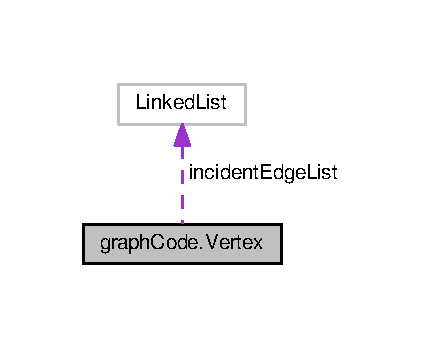
\includegraphics[width=204pt]{classgraphCode_1_1Vertex__coll__graph}
\end{center}
\end{figure}
\subsection*{Public Member Functions}
\begin{DoxyCompactItemize}
\item 
\hyperlink{classgraphCode_1_1Vertex_a470d9de4897ec4d51766d95eedc6e98a}{Vertex} (Object data, Object name)
\item 
Object \hyperlink{classgraphCode_1_1Vertex_ab2e6c18e984280792043a0c7a15e8dca}{get\+Name} ()
\item 
Object \hyperlink{classgraphCode_1_1Vertex_a642a8be0bde891ee0118c54603b3de59}{get\+Data} ()
\item 
void \hyperlink{classgraphCode_1_1Vertex_ac53a68a138244f686f1b2d1d5cff0d7f}{set\+Data} (Object data)
\end{DoxyCompactItemize}


\subsection{Detailed Description}
Class that represents a vertex in a graph. A name (usually a string, but it can be an arbitrary object) can be associated with the vertex.

Data (also represented by an object (e.\+g., a string)) can also be associated with a vertex. This could be useful, for example, if you need to mark a vertex as being visited in some graph traversal.

\begin{DoxyAuthor}{Author}
edhong 
\end{DoxyAuthor}
\begin{DoxyVersion}{Version}
0.\+0 
\end{DoxyVersion}


\subsection{Constructor \& Destructor Documentation}
\index{graph\+Code\+::\+Vertex@{graph\+Code\+::\+Vertex}!Vertex@{Vertex}}
\index{Vertex@{Vertex}!graph\+Code\+::\+Vertex@{graph\+Code\+::\+Vertex}}
\subsubsection[{\texorpdfstring{Vertex(\+Object data, Object name)}{Vertex(Object data, Object name)}}]{\setlength{\rightskip}{0pt plus 5cm}graph\+Code.\+Vertex.\+Vertex (
\begin{DoxyParamCaption}
\item[{Object}]{data, }
\item[{Object}]{name}
\end{DoxyParamCaption}
)\hspace{0.3cm}{\ttfamily [inline]}}\hypertarget{classgraphCode_1_1Vertex_a470d9de4897ec4d51766d95eedc6e98a}{}\label{classgraphCode_1_1Vertex_a470d9de4897ec4d51766d95eedc6e98a}
Constructor that allows data and a name to be associated with the vertex. 
\begin{DoxyParams}{Parameters}
{\em data} & an object to be associated with this vertex \\
\hline
{\em name} & a name to be associated with this vertex \\
\hline
\end{DoxyParams}


\subsection{Member Function Documentation}
\index{graph\+Code\+::\+Vertex@{graph\+Code\+::\+Vertex}!get\+Data@{get\+Data}}
\index{get\+Data@{get\+Data}!graph\+Code\+::\+Vertex@{graph\+Code\+::\+Vertex}}
\subsubsection[{\texorpdfstring{get\+Data()}{getData()}}]{\setlength{\rightskip}{0pt plus 5cm}Object graph\+Code.\+Vertex.\+get\+Data (
\begin{DoxyParamCaption}
{}
\end{DoxyParamCaption}
)\hspace{0.3cm}{\ttfamily [inline]}}\hypertarget{classgraphCode_1_1Vertex_a642a8be0bde891ee0118c54603b3de59}{}\label{classgraphCode_1_1Vertex_a642a8be0bde891ee0118c54603b3de59}
Return the data associated with this vertex. \begin{DoxyReturn}{Returns}
the data of this vertex 
\end{DoxyReturn}
\index{graph\+Code\+::\+Vertex@{graph\+Code\+::\+Vertex}!get\+Name@{get\+Name}}
\index{get\+Name@{get\+Name}!graph\+Code\+::\+Vertex@{graph\+Code\+::\+Vertex}}
\subsubsection[{\texorpdfstring{get\+Name()}{getName()}}]{\setlength{\rightskip}{0pt plus 5cm}Object graph\+Code.\+Vertex.\+get\+Name (
\begin{DoxyParamCaption}
{}
\end{DoxyParamCaption}
)\hspace{0.3cm}{\ttfamily [inline]}}\hypertarget{classgraphCode_1_1Vertex_ab2e6c18e984280792043a0c7a15e8dca}{}\label{classgraphCode_1_1Vertex_ab2e6c18e984280792043a0c7a15e8dca}
Return the name associated with this vertex. \begin{DoxyReturn}{Returns}
the name of this vertex 
\end{DoxyReturn}
\index{graph\+Code\+::\+Vertex@{graph\+Code\+::\+Vertex}!set\+Data@{set\+Data}}
\index{set\+Data@{set\+Data}!graph\+Code\+::\+Vertex@{graph\+Code\+::\+Vertex}}
\subsubsection[{\texorpdfstring{set\+Data(\+Object data)}{setData(Object data)}}]{\setlength{\rightskip}{0pt plus 5cm}void graph\+Code.\+Vertex.\+set\+Data (
\begin{DoxyParamCaption}
\item[{Object}]{data}
\end{DoxyParamCaption}
)\hspace{0.3cm}{\ttfamily [inline]}}\hypertarget{classgraphCode_1_1Vertex_ac53a68a138244f686f1b2d1d5cff0d7f}{}\label{classgraphCode_1_1Vertex_ac53a68a138244f686f1b2d1d5cff0d7f}
Set the data associated with this vertex. 
\begin{DoxyParams}{Parameters}
{\em data} & the data of this vertex \\
\hline
\end{DoxyParams}


The documentation for this class was generated from the following file\+:\begin{DoxyCompactItemize}
\item 
/home/anisha/\+Algo\+Project/\+Network\+Flow\+Study/src/graph\+Code/Vertex.\+java\end{DoxyCompactItemize}

%--- End generated contents ---

% Index
\backmatter
\newpage
\phantomsection
\clearemptydoublepage
\addcontentsline{toc}{chapter}{Index}
\printindex

\end{document}
